% Generated by code/flatten_tex.py; edit main.tex and sections instead.
\documentclass[11pt,a4paper]{article}
\usepackage[T1]{fontenc}
\usepackage[utf8]{inputenc}
\usepackage{lmodern}
\usepackage[a4paper,top=27mm,bottom=27mm,left=27mm,right=27mm,headheight=15pt]{geometry}
\usepackage{amsmath,amssymb,amsthm,mathtools,mathrsfs}
\usepackage{microtype,booktabs,array,longtable,tabularx,enumitem}
\usepackage{graphicx,xcolor,fancyhdr,needspace}
\usepackage[hyphens]{url}
\usepackage[colorlinks=true,linkcolor=midnightblue,citecolor=midnightblue,urlcolor=midnightblue]{hyperref}
\usepackage{bookmark}
\definecolor{midnightblue}{RGB}{26,58,82}
\definecolor{quietgray}{RGB}{85,92,101}
\hypersetup{pdftitle={Formal Reductions and Singular Limits in Polylogarithm Arithmetic},pdfauthor={Research continuation for the ProveIt project},pdfsubject={Cyclotomic rank theorems, Herglotz reductions, Lerch zeros, and angular asymptotics},pdfkeywords={polylogarithms, double shuffle, Herglotz function, Stieltjes constants, Lerch transcendent, asymptotic expansion}}
\newtheorem{theorem}{Theorem}[section]
\newtheorem{lemma}[theorem]{Lemma}
\newtheorem{proposition}[theorem]{Proposition}
\newtheorem{corollary}[theorem]{Corollary}
\theoremstyle{definition}
\newtheorem{definition}[theorem]{Definition}
\newtheorem{conjecture}[theorem]{Conjecture}
\theoremstyle{remark}
\newtheorem{remark}[theorem]{Remark}
\newtheorem{question}[theorem]{Question}
\numberwithin{equation}{section}
\DeclareMathOperator{\Li}{Li}
\DeclareMathOperator{\Imag}{Im}
\DeclareMathOperator{\Rea}{Re}
\DeclareMathOperator{\Gal}{Gal}
\DeclareMathOperator{\rank}{rank}
\newcommand{\Q}{\mathbb Q}
\newcommand{\R}{\mathbb R}
\newcommand{\C}{\mathbb C}
\newcommand{\Z}{\mathbb Z}
\newcommand{\ii}{\mathrm i}
\setlist{itemsep=3pt,topsep=5pt,parsep=0pt}
\setlength{\parindent}{1.3em}
\setlength{\parskip}{2pt}
\setlength{\emergencystretch}{1.5em}
\allowdisplaybreaks[2]
\pagestyle{fancy}
\fancyhf{}
\fancyhead[L]{\small\textcolor{quietgray}{Polylogarithm arithmetic}}
\fancyhead[R]{\small\textcolor{quietgray}{Research continuation \textbullet\ 10 October 2026}}
\fancyfoot[C]{\thepage}
\renewcommand{\headrulewidth}{0.3pt}
\renewcommand{\footrulewidth}{0pt}
\begin{document}
\hypersetup{pageanchor=false}
\begin{titlepage}
\thispagestyle{empty}
\setlength{\parindent}{0pt}
\vspace*{12mm}
{\small\scshape\textcolor{midnightblue}{ProveIt \quad Analysis / Polylogarithms}\par}
\vspace{9mm}
{\LARGE\bfseries\textcolor{midnightblue}{Formal Reductions and Singular Limits\\[3mm] in Polylogarithm Arithmetic}\par}
\vspace{8mm}
{\large Cyclotomic coefficient ranks, rational Herglotz values,\\[1mm]
Lerch zero geometry, and complete angular asymptotics\par}
\vspace{12mm}
{\normalsize A research continuation prepared for Vladimir Reshetnikov\par}
\vspace{2mm}
{\normalsize 10 October 2026\par}
\vspace{13mm}
\begin{abstract}
We continue the ProveIt polylogarithm manuscript at a fixed repository
snapshot, distinguishing newly proved results from recently completed
incoming research. We prove its odd-weight Gaussian coefficient-rank
conjecture, determine the even-weight ranks, and construct a canonical
same-point splitting at every cyclotomic level. For the companion
Herglotz integral $J(p/q)$, we give a complete rational-dilogarithm and
logarithmic classification in the manuscript's rationalized five-term
calculus, together with explicit positive-real evaluations. For
differentiated Lerch logarithmic sums, we classify every small-parameter
zero pattern, prove the optimal uniform threshold $K_2=1$, exhibit a
nonmonotone zero branch, and compute the first singular Abel coefficient
and the exact endpoint regularity of simple zero branches. Finally,
we construct the angular-zero expansion to every exponential order,
uniformly in the second index, and prove that its untruncated series
diverges at every fixed first index. Exact coefficient generators, rational sign certificates, independent numerical diagnostics, a narrow
editorial patch, and a proposed research program accompany the proofs.
Formal relation ranks and five-term obstructions are kept distinct from
unproved independence statements about numerical periods.
\end{abstract}
\vfill
{\small\textcolor{quietgray}{Source baseline: ProveIt commit
\texttt{a2a4cf58c49c745058c40e4a6748d472a3420f18}.\\[2mm]
AI-assisted research preparation; proofs and verification scope are
documented explicitly. This article is an additive research contribution
for review and integration.}\par}
\end{titlepage}
\pagenumbering{roman}
\hypersetup{pageanchor=true}
\tableofcontents
\clearpage
\pagenumbering{arabic}
% BEGIN sections/introduction
\section{Scope, antecedents, and principal results}
\label{intro:sec:scope}

The starting point is the manuscript in
\path{Analysis/Polylogarithms/docs/manuscript} of the ProveIt repository,
at commit \texttt{a2a4cf58c49c745058c40e4a6748d472a3420f18}
\cite{ProveItSnapshot}. The associated incoming reports were inspected
at the same commit. This matters mathematically: several questions that
still appear open in older chapter text have already been answered in
those reports. In particular, the Gaussian weight-five and weight-six
reductions, the residual level-three and level-four polynomial spaces,
and the Möbius-duality certificate for $S_4$ are antecedents, not results
newly established here \cite{PriorResearch,PriorRigidity}.

The continuation develops four connected directions. Each replaces a
finite observation or a qualitative boundary statement by an exact
structural result. Polynomial symmetry determines an infinite family of
matrix ranks. Exterior symbols determine the formal reduction type of
every positive rational Herglotz argument. A singular perturbation
analysis explains why real zeros disappear near the elementary Lerch
endpoint and why the surviving branches need not be monotone. Finite
Lagrange inversion gives the entire exponential scale of an angular
zero, while a separate argument shows that the resulting infinite
expansion is necessarily divergent.

\subsection{Four different meanings of an exact assertion}

We use the following distinctions throughout.
\begin{enumerate}
\item An \emph{analytic identity} is an equality of specified functions
or numbers, with domains, branches, constants, and limiting operations
fixed. The explicit formulas for $J(3/5)$ and $J(n/(n+1))$ have this
meaning.
\item A \emph{coefficient-rank theorem} concerns a fully specified
rational matrix generated by shuffle and stuffle rows. Its kernel is
not a space of numerical periods. A complete answer for that matrix
does not exclude identities arising from additional relations.
\item A \emph{formal dilogarithm classification} concerns the
rationalized pre-Bloch group and its boundary map. A nonzero obstruction
excludes a reduction in that calculus. It does not prove that a
numerical coincidence between periods is impossible.
\item An \emph{exact certificate} is a finite rational or integer
calculation; when it certifies an infinite analytic expression, it is
accompanied by a stated error theorem. Floating-point root
plots and high-precision identity checks are supplementary diagnostics;
they are never used as substitutes for the analytic proofs.
\end{enumerate}
These distinctions allow strong completeness statements without
silently assuming transcendence or period conjectures.

\subsection{The rank conjecture and its universal extension}

The source's Conjecture \texttt{signed:conj:rank} uses $6w-7$ imaginary
depth-two coordinates at fourth roots of unity. It removes the divergent
coordinate and retains a single regularized difference at the boundary.
Theorem~\ref{fg:thm:rank} proves both proposed odd-weight ranks and also
gives the even-weight answer. More significantly, Theorem
\ref{fg:thm:kernel} describes the entire kernel through two freely
chosen homogeneous polynomials. The previously unresolved issue is the
canonical lift of the same-point polynomial through the precise
boundary convention; a rank fit in low weights cannot supply this step.

Theorem~\ref{fg:thm:universal} shows that the lift is independent of the
cyclotomic level. It splits off one explicit antireflection sector for
each conjugate pair of nonreal roots. At level three, combining this
new lift with the earlier residual invariant ring gives the full ranks.
The results provide exact separating functionals for proposed rows,
as well as completeness of the same-point rows in the stated system.
They should be compared with the broader standard relations studied
by Zhao \cite{Zhao2010} and with parity reductions
\cite{Panzer2017,Umezawa2025}; none of those broader theories is being
identified with this restricted single-product matrix.

\subsection{All rational arguments of the Herglotz companion}

Let
\[
J(x)=\int_0^1\frac{\log(1+t^x)}{1+t}\,dt,\qquad x>0.
\]
For reduced $p/q$ with both entries odd, Theorem
\ref{jnew:thm:classification} proves that a formal rational-dilogarithm
reduction exists precisely when $p,q\in\{1,3,5\}$. A formal logarithmic
reduction in this parity class occurs only at $p=q=1$. If $e$ is the
even entry and $o$ the odd entry, the two reduction types coincide and
are characterized by
\[
e^2\equiv\pm1\pmod o,\qquad o^2\equiv1\pmod{2e}.
\]
The doubled modulus is essential. The proof adds a proper-real-subfield
faithfulness theorem for an individual cyclotomic symbol and an exact
dyadic norm identity to the source's all-conductor Gram theorem.

The analytic evaluation section fixes the logarithmic and $\pi^2$
terms suppressed by the formal notation. It derives an explicit
log-sine formula for every consecutive rational argument and obtains
\[
\begin{aligned}
J(3/5)={}&\Li_2(1/3)-\tfrac12\Li_2(1/5)-\tfrac{7\pi^2}{180}
 +\tfrac12\log^2 2+\tfrac12\log^2 3\\
&-\tfrac14\log^2 5+\log^2\left(\tfrac{1+\sqrt5}{2}\right).
\end{aligned}
\]
The functional equations of Radchenko--Zagier and Choie--Kumar are
credited explicitly \cite{RadchenkoZagier,ChoieKumar2023}. The finite
difference used here is a reformulation of known functional equations,
not a claimed new general functional equation. The classifications and
explicit specializations are the contributions of this continuation.

\subsection{Zero geometry at both Lerch endpoints}

For $n,k\geq1$, the normalized differentiated logarithmic Lerch sum is
\[
G_{n,k}(a,\rho)=\sum_{m\geq0}\rho^m
\frac{P_{n,k}(-\log(a+m))}{(a+m)^{k+1}},\qquad a>0,\quad 0\leq\rho\leq1.
\]
The polynomial $P_{n,k}$ is explicit. At $\rho=0$ it may have a
multiple zero at $a=1$. Theorem~\ref{lerchboundary:thm:smallrho}
resolves that zero into convergent Puiseux branches and gives the exact
number of positive zeros for every fixed $n,k$ and all sufficiently
small positive $\rho$. A common compact zero region proves that the
local analysis captures every positive zero.

For $n=2$ we go further: there are exactly two simple positive zeros
for every $k\geq1$ and every $\rho\in[0,1]$. Thus the source's uniform
saturation threshold has the sharp value $K_2=1$. At $k=1$ the smaller
zero first moves below $1$ and ends above $1$, so it is nonmonotone.
The larger branch is strictly decreasing; the smaller branch crosses
$1$ exactly once in the interior and increases thereafter.
At the opposite endpoint, a universal term
$\tau^k\log^{n+1}(1/\tau)$, with $\tau=-\log\rho$, makes every simple
endpoint zero exactly $C^{k-1}$ and not $C^k$. For the two $n=2,k=1$
branches the slopes tend respectively to $+\infty$ and $-\infty$.

\subsection{Every angular scale, and why the series diverges}

Let $\theta_{a,b}$ be the source's unique zero of
$\Imag\Li_{a,b}(e^{\ii\theta},1)$ in the upper semicircle. We construct
the expansion of $\delta_{a,b}=\pi/2-\theta_{a,b}$ to any prescribed
exponential accuracy, uniformly for all real $b>0$. Its scales are
products of the rational numbers $2/n$, $n\geq3$, and its coefficients
are exact polynomials in generalized harmonic numbers. Every cutoff
requires only finitely many coefficients. Ten explicit terms and a
sharp signed remainder are tabulated.

The final asymptotic theorem also clarifies what ``complete'' means.
At each fixed $a,b$, a prime-indexed subsequence of the grouped terms
does not even tend to zero. Consequently the infinite series cannot
be summed by ordinary convergence, although every fixed exponential
cutoff is rigorously asymptotic as $a\to\infty$. This is a concrete
example in which exact, arbitrarily long expansions coexist with
unavoidable divergence.

\subsection{Dependencies and reproducibility}

The matrix proofs and angular coefficient construction are algebraic
and analytic arguments valid in all weights. The Herglotz classification
uses the source's proved Gram theorem and its explicitly stated
rationalized Bloch-group facts. The zero results use the source's
global variation bound and eleven replayed rational endpoint signs;
the essential background and the variation argument are recalled here.
Only the nonvanishing of a polynomial at $-\log2$ uses classical
Hermite--Lindemann transcendence.

The source manifest, scripts, output receipts, and a claim ledger are
included with the article. New proofs received independent internal
mathematical cross-checks. No claim of formal proof-assistant
verification or external peer review is made. The remaining questions
are listed with concrete next steps in Section~\ref{research:sec:program}.
% END sections/introduction
% BEGIN sections/gaussian_rank
% Research contribution for integration into the parent article.
% Requires amsmath, amssymb, amsthm, booktabs, and theorem/lemma/corollary environments.
% All labels use the prefix fg:.
\section{The full Gaussian single-product rank conjecture}
\label{fg:sec:rank}

The manuscript's Conjecture~\texttt{signed:conj:rank} concerns a precise
coefficient matrix, rather than the dimension of a space of actual
polylogarithmic numbers. We prove both proposed rank formulas in every
odd weight. The proof also gives the full even-weight answer, an explicit
basis of the nullspace, and a complete finite test for whether an arbitrary
coefficient vector follows from the stated rows.

The additional boundary issue is essential. A preceding incoming report,
\path{polylogarithms_research_2026-10-10.zip}, proves the dimension after
setting the Gaussian family to zero and after retaining regularized rows
in a different presentation. Our result keeps that family free, removes
exactly the manuscript's divergent coordinate, and retains only the
stuffle-minus-shuffle difference when a single factor diverges. The new
step is a canonical lift of every allowed Gaussian nullvector through
that precise boundary presentation.

\subsection{The matrix and its scope}

Fix an integer $w\ge2$ and write $n=w-2$. For $a+b=w$, let
\[
 D_{a,b}(x,y)=\sum_{k>\ell>0}\frac{x^ky^\ell}{k^a\ell^b},
 \qquad X_a^{r,s}=\operatorname{Im}D_{a,w-a}(i^r,i^s),
 \quad r,s\in\mathbb Z/4\mathbb Z.
\]
For the coefficient computation, the $X_a^{r,s}$ are formal rational
coordinates. Impose conjugation
$X_a^{-r,-s}=-X_a^{r,s}$ and put $X_a^{r,s}=0$ if both colors are even.
A set of representatives of the remaining color pairs is
\begin{equation}\label{fg:eq:pairs}
 (0,1),\ (1,0),\ (1,1),\ (1,2),\ (1,3),\ (2,1).
\end{equation}
Remove $X_1^{0,1}$, the single divergent imaginary coordinate in these
representatives. Thus the ambient coefficient space has dimension
$N_w=6(w-1)-1=6w-7$.

For $p+q=w$ and $r,s\in\mathbb Z/4\mathbb Z$, define the stuffle and
shuffle coefficient rows
\begin{align}
 S_{p,q}^{r,s}
 &=X_p^{r,s}+X_q^{s,r},\\
 H_{p,q}^{r,s}
 &=\sum_{j=0}^{p-1}\binom{q+j-1}{j}X_{q+j}^{s,r-s}
   +\sum_{j=0}^{q-1}\binom{p+j-1}{j}X_{p+j}^{r,s-r}.
 \label{fg:eq:raw-rows}
\end{align}
If both single factors $\operatorname{Li}_p(i^r)$ and
$\operatorname{Li}_q(i^s)$ are finite, retain the two rows separately.
If exactly one factor is $\operatorname{Li}_1(1)$, retain only
$S_{p,q}^{r,s}-H_{p,q}^{r,s}$, in which the removed coordinate cancels.
The two-divergent-factor case occurs only at $w=2$ with two real colors;
its imaginary coefficient row is zero. Discard zero rows; retaining
repeated rows does not change the problem. Call the resulting rational
matrix $A_w$. Let $A_w^{\neg g}$ be obtained by deleting the $w-1$
columns $X_a^{1,0}$.

The depth-one right sides are suppressed because the present question
concerns the coefficient row space. Analytically, these rows come from
convergent shuffle and stuffle identities, and from subtracting the
one-divergence identities before taking a regularized limit. Nothing
here assigns a value to $\zeta(1)$. This is a restricted linear system
of products of two depth-one values. In particular, it omits distribution,
higher-depth products and elimination, and additional argument
transformations. It is narrower than the families of standard relations
studied by Zhao; see J.~Zhao, \emph{Standard Relations of Multiple
Polylogarithm Values at Roots of Unity}, Documenta Mathematica
\textbf{15} (2010), 1--34, \texttt{arXiv:0707.1459}.

\begin{theorem}[Exact ranks in every weight]\label{fg:thm:rank}
The matrix family just defined satisfies
\begin{align}
 \operatorname{rank}_{\mathbb Q}A_w
 &=\begin{cases}
      6w-7,&w\text{ even},\\
      5w-6,&w\text{ odd},
    \end{cases}\label{fg:eq:full-rank}\\
 \operatorname{rank}_{\mathbb Q}A_w^{\neg g}
 &=\begin{cases}
      5w-6,&w\text{ even},\\
      (9w-11)/2,&w\text{ odd}.
    \end{cases}\label{fg:eq:nong-rank}
\end{align}
In particular, both equalities in the manuscript's odd-weight rank
conjecture hold for every odd $w\ge3$.
\end{theorem}

The proof is an explicit description of the entire kernel. It does not
extrapolate from finite rank calculations.

\subsection{Encoding the rows by homogeneous polynomials}

For a scalar assignment to the formal coordinates, set
\[
 \mathscr F^{r,s}(X,Y)
   =\sum_{a=1}^{w-1}X_a^{r,s}X^{a-1}Y^{w-a-1}.
\]
These homogeneous polynomials have degree $n$. Write
\[
 U=\mathscr F^{0,1},\quad G=\mathscr F^{1,0},\quad
 A=\mathscr F^{1,1},\quad K=\mathscr F^{1,2},\quad
 M=\mathscr F^{1,3},\quad V=\mathscr F^{2,1}.
\]
The letter $A$ in these formulas denotes a polynomial; the matrix is
always written $A_w$. The removed coordinate is encoded by
\begin{equation}\label{fg:eq:removed}
 [Y^n]U(X,Y)=0.
\end{equation}
For a polynomial $P$, let $P^\sigma(X,Y)=P(Y,X)$.

Coefficient comparison turns a complete set of finite stuffle rows into
$\mathscr F^{r,s}(X,Y)+\mathscr F^{s,r}(Y,X)=0$. Similarly, the shuffle
rows are the coefficients of
\[
 \mathscr F^{s,r-s}(X+Y,X)
   +\mathscr F^{r,s-r}(X+Y,Y).
\]
For example, the coefficient of $X^{p-1}Y^{q-1}$ in the second summand
is precisely the second binomial sum in
\eqref{fg:eq:raw-rows}. This explains the substitutions without invoking
any rank or transcendence theorem.

\begin{lemma}[The boundary defect]\label{fg:lem:boundary}
Put $c=[X^n]G(X,Y)$. The finite rows with product colors $(0,1)$,
together with their one-divergence difference row, are exactly
\begin{align}
 U(X,Y)+G(Y,X)&=cY^n,\\
 M(X+Y,X)+U(X+Y,Y)&=cY^n.
 \label{fg:eq:boundary}
\end{align}
Consequently they determine
\begin{equation}\label{fg:eq:UM}
 U(X,Y)=-G(Y,X)+cY^n,
 \qquad M(X,Y)=G(X-Y,X).
\end{equation}
\end{lemma}
\begin{proof}
For colors $(0,1)$, the factor $\operatorname{Li}_p(1)$ is finite
exactly when $p\ge2$. Therefore the coefficients of
$X^{p-1}Y^{q-1}$ in the stuffle polynomial
$U(X,Y)+G(Y,X)$ vanish for all $p\ge2$. The only possible defect is
a multiple of $Y^n$. By \eqref{fg:eq:removed}, its coefficient is $c$.
The same finite-product argument shows that
$M(X+Y,X)+U(X+Y,Y)$ has only a $Y^n$ defect, say $dY^n$.
When $p=1$, the retained regularized row is the difference of these
two coefficient rows. It says exactly $c-d=0$. This proves
\eqref{fg:eq:boundary}. Substituting the first identity into the
second cancels $cY^n$ and gives
$M(X+Y,X)=G(Y,X+Y)$. The invertible substitution
$(X+Y,X)\mapsto(X,Y)$ yields \eqref{fg:eq:UM}.
The argument also covers $w=2$: there are no $p\ge2$ coefficients,
and the difference row still equates the two constant defects.
\end{proof}

This lemma is the point at which the precise regularization convention
matters. Setting the two boundary rows separately to zero would impose
an extra condition on $c$. Deleting the boundary row altogether would
lose a condition. The manuscript's difference convention produces the
unique correction $cY^n$.

\begin{lemma}[Exhaustive kernel conditions]\label{fg:lem:conditions}
An assignment annihilates every row of $A_w$ if and only if its six
polynomials satisfy \eqref{fg:eq:UM} and
\begin{align}
 A(Y,X)&=-A(X,Y), & V(X,Y)&=-K(Y,X),\\
 M(Y,X)&=M(X,Y), & G(X,Y)&=-G(X,X-Y),\\
 K(X,Y)&=-A(Y,Y-X),&K(X,Y)&=K(X,X-Y).
 \label{fg:eq:conditions}
\end{align}
\end{lemma}
\begin{proof}
The product-color classes $(1,1),(1,2),(1,3)$ give the conditions in
this table:
\[
\begin{array}{c|c|c}
 \text{colors}&\text{stuffle}&\text{shuffle}\\ \hline
 (1,1)& A+A^\sigma=0
   &G(X+Y,X)+G(X+Y,Y)=0\\
 (1,2)&K+V^\sigma=0
   &A(X+Y,X)-V(X+Y,Y)=0\\
 (1,3)&M-M^\sigma=0
   &K(X+Y,Y)-K(X+Y,X)=0.
\end{array}
\]
For the $(1,2)$ shuffle we have exchanged the two product factors;
this merely transposes $X,Y$ and retains exactly the same collection
of coefficient rows. Substituting $V=-K^\sigma$ into its shuffle gives
$K(X,Y)=-A(Y,Y-X)$. The other two shuffle equations yield the two
reflection equations in \eqref{fg:eq:conditions}.

There are no omitted nonzero color classes. Up to swapping the product
factors and conjugation, all unordered pairs are
\[
 (0,0),\ (0,1),\ (0,2),\ (1,1),\ (1,2),\ (1,3),\ (2,2).
\]
The classes $(0,0),(0,2),(2,2)$ are entirely real and their imaginary
rows vanish. The $(0,1)$ class is exactly
Lemma~\ref{fg:lem:boundary}. This proves necessity and sufficiency.
\end{proof}

\subsection{The two independent polynomial sectors}

\begin{theorem}[Canonical description of the full nullspace]
\label{fg:thm:kernel}
For even $w$, $\ker A_w=0$. For odd $w=2m+1$, its elements are in
one-to-one correspondence with independent choices of degree
$n=2m-1$ homogeneous polynomials $G,A$ satisfying
\begin{equation}\label{fg:eq:two-sectors}
 G(X,Y)=-G(X,X-Y),\qquad A(X,Y)=-A(Y,X).
\end{equation}
All six polynomials are then given by
\begin{align}
 U(X,Y)&=-G(Y,X)+cY^n,&c&=[X^n]G,\\
 M(X,Y)&=G(X-Y,X),\\
 K(X,Y)&=-A(Y,Y-X),\\
 V(X,Y)&=-K(Y,X).
 \label{fg:eq:kernel-map}
\end{align}
Each sector has dimension $m$. In particular,
$\dim\ker A_w=2m=w-1$ at odd weight.
\end{theorem}
\begin{proof}
The preceding lemmas show that every kernel element is of the form
\eqref{fg:eq:kernel-map}, with the two conditions
\eqref{fg:eq:two-sectors}. It remains to impose the symmetry of $M$
and the reflection symmetry of $K$. Homogeneity and the reflection
condition on $G$ give
\begin{align*}
 M(Y,X)&=G(Y-X,Y)
       =(-1)^nG(X-Y,-Y)\\
       &=-(-1)^nG(X-Y,X)
        =(-1)^{n+1}M(X,Y).
\end{align*}
Likewise, antisymmetry of $A$ gives
\begin{align*}
 K(X,X-Y)&=-A(X-Y,-Y)\\
         &=-(-1)^nA(Y-X,Y)
          =(-1)^nA(Y,Y-X)\\
         &=(-1)^{n+1}K(X,Y).
\end{align*}
If $n$ is even, the required equalities $M=M^\sigma$ and
$K(X,Y)=K(X,X-Y)$ force $M=K=0$, hence $G=A=0$, and then all six
polynomials vanish. If $n$ is odd, these two remaining equalities
hold automatically. The exhaustive list of classes in
Lemma~\ref{fg:lem:conditions} proves that every pair in
\eqref{fg:eq:two-sectors} is a kernel element, so this is a bijective
parameterization.

For the $G$ sector, change variables from $X,Y$ to $X,Z=2Y-X$.
Reflection changes $Z$ to $-Z$, so $G$ is an odd polynomial in $Z$.
At total degree $2m-1$, a basis is
\begin{equation}\label{fg:eq:G-basis}
 G_j(X,Y)=X^{2j}(2Y-X)^{2m-1-2j},\qquad 0\le j<m.
\end{equation}
For the $A$ sector, a basis is
\begin{equation}\label{fg:eq:A-basis}
 A_j(X,Y)=X^{2m-1-j}Y^j-X^jY^{2m-1-j},\qquad 0\le j<m.
\end{equation}
Their independence follows respectively from the distinct powers of
$Z$, and from their disjoint exchanged monomial pairs. Thus each
sector has dimension $m$.
\end{proof}

\begin{proof}[Proof of Theorem~\ref{fg:thm:rank}]
The full matrix has $6w-7$ columns. Subtracting the kernel dimensions
in Theorem~\ref{fg:thm:kernel} gives
\eqref{fg:eq:full-rank}. To pass to $A_w^{\neg g}$, extend a vector
on the remaining columns by zero on the deleted Gaussian columns.
It is in $\ker A_w^{\neg g}$ if and only if the extended vector is
in $\ker A_w$ and $G=0$. At odd weight this leaves exactly the
$m$-dimensional $A$ sector; at even weight it leaves zero. There
are $(6w-7)-(w-1)=5w-6$ remaining columns. Subtracting these
kernel dimensions gives \eqref{fg:eq:nong-rank}.
\end{proof}

The Hilbert series of these formal nullspaces are especially simple:
\[
 \sum_{w\ge2}\dim\ker A_w\,t^w
 =\frac{2t^3}{(1-t^2)^2},\qquad
 \sum_{w\ge2}\dim\ker A_w^{\neg g}\,t^w
 =\frac{t^3}{(1-t^2)^2}.
\]
The second is the previously obtained quotient count; the first records
the additional freely liftable Gaussian sector.

\subsection{Every Gaussian-only consequence is already a same-point shuffle}

Let $\mathcal R_w$ be the row space of $A_w$ and let $E_g$ be the
coordinate subspace supported only on the Gaussian columns.
Projection of $\mathcal R_w$ onto the other columns has dimension
$\operatorname{rank}A_w^{\neg g}$. Hence
\begin{equation}\label{fg:eq:intersection}
 \dim(\mathcal R_w\cap E_g)
 =\operatorname{rank}A_w-\operatorname{rank}A_w^{\neg g}
 =\begin{cases}
    w-1,&w\text{ even},\\
    (w-1)/2,&w\text{ odd}.
  \end{cases}
\end{equation}

\begin{corollary}[Completeness for Gaussian-only coefficient rows]
\label{fg:cor:g-only}
For odd $w=2m+1$, every rational linear combination of the defining
rows whose non-Gaussian coefficients cancel is a rational linear
combination of the $m$ same-point product-shuffle rows obtained from
\[
 \operatorname{Li}_p(i)\operatorname{Li}_{w-p}(i),
 \qquad 1\le p\le m.
\]
Thus enlarging a search to all the colors and one-divergence rows in
$A_w$ yields no additional Gaussian-only coefficient relation in
odd weight beyond these elementary shuffles.
\end{corollary}
\begin{proof}
These $m$ rows are present in $A_w$ and are supported only on $G$.
They are independent: in the usual inner-index ordering, the row
with $p\le m$ has largest inner index $q=w-p$, with coefficient
one, and no larger inner index occurs. Ordering the selected rows
and columns accordingly gives a triangular square block with unit
diagonal. Their span is therefore an $m$-dimensional subspace of
$\mathcal R_w\cap E_g$, which also has dimension $m$ by
\eqref{fg:eq:intersection}. The spaces are equal.
\end{proof}

This is a statement about the coefficient projection of the equations.
When actual depth-one right sides are restored, any equality of row
coefficients also gives the corresponding identity of those right
sides, because all the underlying analytic rows are valid. The
corollary does not forbid Gaussian-only identities from other
functional equations or higher-depth elimination.

\subsection{A complete membership test and exact certificates}

Equations \eqref{fg:eq:G-basis}--\eqref{fg:eq:A-basis}, followed by
\eqref{fg:eq:kernel-map}, give $w-1$ explicit integer vectors
$v_1,\ldots,v_{w-1}$ in odd weight. For any rational coefficient row
$t$, elementary finite-dimensional duality gives
\begin{equation}\label{fg:eq:membership}
 t\in\operatorname{rowspan}_{\mathbb Q}A_w
 \quad\Longleftrightarrow\quad
 t\cdot v_j=0\quad\text{for every }j.
\end{equation}
Thus membership in the stated coefficient module has a complete test
using only integer polynomial substitution and rational dot products.
A nonzero dot product supplies a short exact separating functional.
At even weight the row space is the whole coordinate space. None of
these tests asserts the absence of a relation outside this matrix.

At weight five, $n=3$, one may choose
\[
 G_0=(2Y-X)^3,\quad G_1=X^2(2Y-X),\qquad
 A_0=X^3-Y^3,\quad A_1=X^2Y-XY^2.
\]
These four parameters give the four-dimensional nullspace of the
$92\times23$ matrix, with no numerical polylogarithm computation.
The $G$-zero subspace has the two $A$ parameters, explaining the
rank pair $(19,17)$. At weight seven the corresponding pair is
$(29,26)$, and at weight thirty-one it is $(149,134)$.

The supplied standard-library program
\texttt{full\_gaussian\_rank.py} constructs the raw rows from
\eqref{fg:eq:raw-rows}; its separate polynomial code constructs
\eqref{fg:eq:kernel-map}. It verifies that every displayed basis
vector annihilates every raw row. Independent rational elimination
checks both ranks in weights $2$ through $11$. Basis identities are
also replayed in weights $12$ through $17$ and in weights
$23,31,47,63$. The JSON receipt includes the entire weight-five
matrix, coordinate order, row labels, and kernel basis. These finite
checks validate the implementation; the preceding proof establishes
all weights.

\subsection{Integration notes and further questions}

The manuscript's Conjecture~\texttt{signed:conj:rank} can be replaced
by Theorem~\ref{fg:thm:rank}. The even-weight formulas and the
canonical kernel description are additional results. The word
``equivalently'' preceding the manuscript's row-space-intersection
formulation should be changed to ``consequently,'' unless one of
the absolute rank formulas is taken as an additional premise: a
specified difference of two ranks does not by itself determine both
ranks. Our proof establishes the absolute ranks and their difference.

Three directions now have precise formulations. First, replace the
implicit numerical rank routine by the explicit polynomial test
\eqref{fg:eq:membership} in future relation searches. Second, add
specified distribution or octahedral rows and compute their action
on these two small polynomial sectors, rather than repeating
elimination in all $6w-7$ coordinates. Third, classify which
higher-depth relations couple the two sectors. Such a classification
would address a larger relation module; passing from any formal
module to numerical period independence remains a separate problem.
% END sections/gaussian_rank
% BEGIN sections/universal_lift
% Optional continuation of full_gaussian_rank.tex; same theorem environments.
\section{A universal splitting at every cyclotomic level}
\label{fg:sec:universal}

The boundary lift used above does not depend on the number four. It
separates the same-point coordinates from the remaining color problem
at every cyclotomic level.

Let $N\ge3$, $\omega=e^{2\pi i/N}$, and define the formal imaginary
coordinates for $D_{a,w-a}(\omega^r,\omega^s)$ exactly as before, now
with colors modulo $N$. Impose conjugation, discard its fixed
coordinates, and remove one divergent coordinate $X_1^{0,r}$ for
each conjugate pair of nonreal roots. Let $A_{N,w}$ be the matrix of
finite single-product shuffle and stuffle rows, with only their
difference retained when exactly one factor diverges. Put
\[
 R_N=\{1,\ldots,\lfloor(N-1)/2\rfloor\},\qquad k_N=|R_N|.
\]
The matrix has
\[
 d_{N,w}=\frac{N^2-\gcd(N,2)^2}{2}(w-1)-k_N
\]
columns: conjugation has $\gcd(N,2)^2$ fixed color pairs, and the
last term counts the removed divergent coordinates. Let
$A_{N,w}^{\neg g}$ delete all $k_N(w-1)$ same-point columns
$X_a^{r,0}$ with $r\in R_N$. These are formal matrices with the same
restricted meaning as $A_w$; distribution and higher-depth rows
have not been added.

For a homogeneous degree-$n$ polynomial, where $n=w-2$, define
\[
 \mathcal H_n^-=
 \{G\in\mathbb Q[X,Y]_n:G(X,Y)=-G(X,X-Y)\}.
\]

\begin{theorem}[Universal same-point splitting]\label{fg:thm:universal}
For odd $w=2m+1$, there is a canonical split exact sequence
\[
 0\longrightarrow\ker A_{N,w}^{\neg g}
 \longrightarrow\ker A_{N,w}
 \longrightarrow\bigoplus_{r\in R_N}\mathcal H_{2m-1}^-
 \longrightarrow0.
\]
The last map records the same-point polynomials $G_r$.
In particular,
\begin{equation}\label{fg:eq:universal-nullity}
 \dim\ker A_{N,w}-\dim\ker A_{N,w}^{\neg g}=k_Nm.
\end{equation}
At even $w$, every vector in $\ker A_{N,w}$ has all same-point
coordinates zero, so the two kernels are naturally identical.
Consequently
\begin{equation}\label{fg:eq:universal-rank-difference}
 \operatorname{rank}A_{N,w}-\operatorname{rank}A_{N,w}^{\neg g}
 =\begin{cases}
    k_N(w-1),&w\text{ even},\\
    k_N(w-1)/2,&w\text{ odd}.
  \end{cases}
\end{equation}
\end{theorem}
\begin{proof}
Fix $r\in R_N$ and abbreviate the polynomials for colors
$(r,0),(0,r),(r,-r)$ by $G_r,U_r,M_r$. The product-color classes
$(r,r),(0,r),(r,-r)$ imply exactly the same necessary conditions
as in the Gaussian proof:
\begin{align*}
 G_r(X,Y)&=-G_r(X,X-Y),\\
 U_r(X,Y)&=-G_r(Y,X)+c_rY^n,\qquad c_r=[X^n]G_r,\\
 M_r(X,Y)&=G_r(X-Y,X),\qquad M_r=M_r^\sigma.
\end{align*}
The boundary equation uses the single regularized difference,
so its derivation is unchanged. Homogeneity gives
$M_r^\sigma=(-1)^{n+1}M_r$. Thus even $n$ forces $G_r=0$.
For odd $n$, the symmetry of $M_r$ is automatic.

For odd $n$, define a section by assigning the displayed values to
these three color pairs for each $r$, their negatives to conjugate
pairs, and zero to every other color pair. This assignment satisfies
all rows. Here is a support check that prevents an implicit assumption
about the other colors. A shuffle can meet a nonzero $G_r$ coordinate
only when its two product colors are $(r,r)$, and then it is exactly
the antireflection equation. It can meet $U_r$ or $M_r$ only for
product colors $(0,r)$ or $(r,0)$, and then it is exactly the boundary
equation. The stuffle rows meeting these coordinates are the boundary
class and $(r,-r)$, which is the symmetry of $M_r$. Transposition
and conjugation cover the reversed and conjugate classes. Thus no
unexamined row couples the proposed section to other colors.
The supports for distinct $r\in R_N$ are disjoint.

Subtracting this section from any kernel vector leaves all $G_r=0$;
the remainder is naturally a vector in $\ker A_{N,w}^{\neg g}$.
This proves the splitting. Since
$\dim\mathcal H_{2m-1}^-=m$, it gives
\eqref{fg:eq:universal-nullity}. Subtracting kernel dimensions from
column counts proves \eqref{fg:eq:universal-rank-difference}.
\end{proof}

At odd weight, an immediate consequence is that every coefficient
relation supported only on these same-point columns is spanned by
the independent same-point shuffle rows, separately for each root
pair. Those rows already supply $k_N(w-1)/2$ dimensions, equal to
\eqref{fg:eq:universal-rank-difference}. Thus the Gaussian-only
completeness result above is one instance of a level-independent
fact about this particular single-product coefficient system.

\subsection{The complete level-three ranks}

The earlier incoming report \cite{PriorResearch} already identifies the residual
level-three space after $G=0$. In that case the boundary formulas
force $U=M=0$, so its regularized presentation and the present
removed-coordinate presentation agree. Its remaining polynomial
satisfies
\[
 A(Y,X)=-A(X,Y),\qquad A(X,X-Y)=A(X,Y),
\]
and is parameterized by
\[
 A=\Delta\,\mathbb Q[Q,\Delta^2],\qquad
 \Delta=XY(X-Y),\quad Q=X^2-XY+Y^2.
\]
At odd weight its homogeneous degree-$w-2$ component has dimension
$\lfloor(w+1)/6\rfloor$, and at even weight it is zero.
For completeness, antisymmetry and reflection force the three
linear factors of $\Delta$; after their removal the quotient is
invariant under the group generated by the two transformations.
That group acts as permutations and global negation on
$(X,-Y,Y-X)$, whose sum is zero, giving the invariant ring
$\mathbb Q[Q,\Delta^2]$. Counting monomials of degrees
$3+2a+6b=w-2$ gives the stated dimension.
This residual description is credited to the preceding report; the
new assertion is its extension to the free same-point family under
the manuscript's boundary convention.

\begin{corollary}[Level-three extension]\label{fg:cor:level3}
The analogous full level-three matrix has $4w-5$ columns and satisfies
\[
 \operatorname{rank}A_{3,w}
 =\begin{cases}
    4w-5,&w\text{ even},\\
    (7w-9)/2-\lfloor(w+1)/6\rfloor,&w\text{ odd},
  \end{cases}
\]
while the matrix with all same-point columns deleted satisfies
\[
 \operatorname{rank}A_{3,w}^{\neg g}
 =\begin{cases}
    3w-4,&w\text{ even},\\
    3w-4-\lfloor(w+1)/6\rfloor,&w\text{ odd}.
  \end{cases}
\]
\end{corollary}
\begin{proof}
At odd weight the full kernel has dimension
$(w-1)/2+\lfloor(w+1)/6\rfloor$ by
Theorem~\ref{fg:thm:universal}; its restricted kernel has only the
second summand. Both vanish at even weight. Subtraction from the
respective column counts proves the formulas.
\end{proof}

The supplementary program \texttt{universal\_gaussian\_lift.py}
verifies the lift directly against every raw row at selected weights
and levels $3,4,5,6,8,10,12$. Independent exact ranks in weights
$2,3,4$ at levels $3$ through $6$ check the rank differences. This
establishes neither a formula for the remaining kernel at arbitrary
level nor numerical period independence; those remain separate
questions.
% END sections/universal_lift
% BEGIN sections/herglotz_classification
% Research contribution for the pinned ProveIt manuscript.
% Standard theorem environments and amsmath/amssymb are assumed.
\section{A complete formal classification of rational companion values}
\label{jnew:sec:classification}

Put
\[
 J(x)=\int_0^1\frac{\log(1+t^x)}{1+t}\,dt,
 \qquad
 F(x)=\sum_{n\ge1}\frac{\psi(nx)-\log(nx)}n.
\]
Radchenko--Zagier's identity~\cite{RadchenkoZagier} is
\begin{equation}\label{jnew:eq:JF}
 J(x)=F(2x)-2F(x)+F(x/2)+\frac{\pi^2}{12x}.
\end{equation}
All identities in this section at positive real arguments use real logarithms.
Our negative statements concern the rationalized five-term calculus, not
numerical independence of periods.

Write $A(K)=K^\times\otimes_{\mathbb Z}\mathbb Q$ additively, using
$\langle u\rangle$ for the class of $u$. Roots of unity disappear.
Let $\mathcal P(K)$ be the rationalized pre-Bloch group, with
$\partial[z]=\langle z\rangle\wedge\langle1-z\rangle$ and
$[0]=[1]=0$. For coprime positive $p,q$, let $\xi_{p/q}$ denote the
Galois-invariant element supplied by the finite cyclotomic formula for
$F(p/q)-F(1)$. Its normalization is
\begin{equation}\label{jnew:eq:xi-boundary}
 \partial\xi_{p/q}
 =\beta_q(p)-\beta_p(q)-\langle p\rangle\wedge\langle q\rangle,
 \qquad
 \beta_m(a)=\sum_{k=1}^{m-1}
 \langle1-\zeta_m^{ak}\rangle\wedge\langle1-\zeta_m^k\rangle.
\end{equation}
Set $\beta_1=\beta_2=0$. Fractions in subscripts are always reduced
before using \eqref{jnew:eq:xi-boundary}. Define
\begin{equation}\label{jnew:eq:eta}
 \eta_{p/q}=\xi_{2p/q}-2\xi_{p/q}+\xi_{p/(2q)}
 \quad\text{in }\mathcal P(\mathbb Q(\zeta_{2pq})).
\end{equation}
A formal logarithmic reduction of $J(p/q)$ means $\eta_{p/q}=0$;
a formal rational-dilogarithm reduction means
$\eta_{p/q}\in\operatorname{im}\mathcal P(\mathbb Q)$.
Products of algebraic logarithms and rational multiples of $\pi^2$
are the terms suppressed by this terminology.

We use the established rationalized facts
\[
 \ker(\partial|_{\mathcal P(K)})^{\operatorname{Gal}(K/\mathbb Q)}=0,
 \qquad
 \partial\mathcal P(\mathbb Q)=\Lambda^2 A(\mathbb Q)
\]
for Galois number fields $K$ \cite[\texttt{hstruct:eq:bloch-facts}]{ProveItSnapshot}. These are the Bloch-group descent and
$K_2(\mathbb Q)$ inputs already used in the manuscript. Consequently,
for an invariant $\eta$, the two kinds of reduction are equivalent,
respectively, to $\partial\eta=0$ and
$\partial\eta\in\Lambda^2 A(\mathbb Q)$.

\subsection{The existing Gram theorem and a new subfield consequence}

For $M\ge3$, set $G_M=(\mathbb Z/M\mathbb Z)^\times/\{\pm1\}$.
The all-conductor Gram theorem of the manuscript
\cite[\texttt{hstruct:thm:kernel}, \texttt{hstruct:lem:positive-Gram}]{ProveItSnapshot}
states that
\begin{equation}\label{jnew:eq:kernel}
 \sum_{a\in G_M}c_a\beta_M(a)=0
 \quad\Longleftrightarrow\quad c_a=c_{a^{-1}}\quad(a\in G_M).
\end{equation}
In particular $\beta_M(a)=0$ precisely when $a^2\equiv\pm1\pmod M$.
Its proof provides more information than this zero test. Put
\[
 v_k=(\log|1-\zeta_M^{bk}|)_{b\in G_M},\qquad
 A_M=\sum_{k=1}^{M-1}v_kv_k^{\mathsf T},\qquad
 (P_av)_b=v_{ba}.
\]
Then $A_M$ is positive definite, commutes with every $P_a$, and the
logarithmic exterior image of $\beta_M(a)$ is
\begin{equation}\label{jnew:eq:Gram-image}
 A_M(P_a-P_{a^{-1}}).
\end{equation}
The positivity uses all roots, including roots of lower order: for a
nontrivial even character of primitive conductor $f\mid M$, the
$k=M/f$ vector has a nonzero Fourier coefficient proportional to
$\tau(\chi)L(1,\overline\chi)$. Prime-order roots supply the trivial
character. This is an exact nonvanishing argument, not a numerical
determinant test. We never assume that the logarithmic exterior map
is injective on the whole exterior square.

\begin{theorem}[No proper real subfield for a nonzero individual symbol]
\label{jnew:thm:subfield}
Let $L=\mathbb Q(\zeta_M)^+$ and let $E$ be a proper subfield of $L$.
If the element $\beta_M(a)$ belongs to the image of
$\Lambda^2 A(E)$ in $\Lambda^2 A(L)$, then $\beta_M(a)=0$.
\end{theorem}
\begin{proof}
The symbols do belong to the real field, because
\[
 \langle1-\zeta_M^k\rangle
 =\tfrac12\langle(1-\zeta_M^k)(1-\zeta_M^{-k})\rangle.
\]
Let $H=\operatorname{Gal}(L/E)$, a nontrivial subgroup of $G_M$.
Logarithmic vectors of elements of $E$ lie in
$W=(\mathbb R^{G_M})^H$. A skew matrix arising from
$\Lambda^2 W$ annihilates $W^\perp$. On the complex character line
of a character $\chi$ nontrivial on $H$, formula
\eqref{jnew:eq:Gram-image} therefore gives
\[
 \lambda_\chi\bigl(\chi(a)-\chi(a)^{-1}\bigr)=0,
 \qquad\lambda_\chi>0.
\]
Thus $\chi(a)^2=1$ for every such character. Let $X_0$ be the
proper subgroup of characters trivial on $H$, and choose
$\chi_0\notin X_0$. For every $\psi\in X_0$, both $\chi_0$ and
$\chi_0\psi$ are outside $X_0$. Dividing their squared values gives
$\psi(a)^2=1$. Thus all characters of $G_M$ are trivial at $a^2$.
Characters separate points, so $a^2=1$ in $G_M$, and
\eqref{jnew:eq:kernel} gives $\beta_M(a)=0$.
\end{proof}

This statement concerns a single $\beta_M(a)$. It does not assert
that every nonzero linear combination of symbols has this property.

\subsection{Two exact dyadic identities}

\begin{lemma}[Odd conductor doubling]\label{jnew:lem:odd-double}
If $m$ is odd and $a$ is odd with $(a,m)=1$, then, inside
$\mathbb Q(\zeta_{2m})=\mathbb Q(\zeta_m)$,
\begin{equation}\label{jnew:eq:odd-double}
 \beta_{2m}(a)=3\beta_m(a)-\beta_m(2a)-\beta_m(a/2),
\end{equation}
where division by $2$ means multiplication by its inverse modulo $m$.
\end{lemma}
\begin{proof}
The even-indexed roots contribute $\beta_m(a)$. Write the odd-indexed
roots as $-\zeta_m^j$, $0\le j<m$. The $j=0$ term is
$\langle2\rangle\wedge\langle2\rangle=0$.
For $j\ne0$, put $u_j=\langle1-\zeta_m^j\rangle$. Factorization gives
$\langle1+\zeta_m^j\rangle=u_{2j}-u_j$. The remaining contribution is
\[
 \sum_{j=1}^{m-1}(u_{2aj}-u_{aj})\wedge(u_{2j}-u_j)
 =2\beta_m(a)-\beta_m(2a)-\beta_m(a/2).
\]
Adding the even-root contribution proves the identity.
\end{proof}

\begin{lemma}[Even conductor second difference]\label{jnew:lem:even-difference}
Let $e\ge2$ be even and $(a,2e)=1$. Put
\[
 \Delta_e(a)=\beta_{2e}(a)-2\beta_e(a)+\beta_{e/2}(a).
\]
Then
\begin{equation}\label{jnew:eq:Delta-zero}
 \Delta_e(a)=0
 \quad\Longleftrightarrow\quad a^2\equiv1\pmod{2e}.
\end{equation}
\end{lemma}
\begin{proof}
For $e=2$ all three symbols vanish and every odd square is $1$
modulo $4$. Suppose $e\ge4$. Let $N$ be the normalized field norm
from $\mathbb Q(\zeta_{2e})$ to $\mathbb Q(\zeta_e)$, acting on
$A$ by division by the extension degree $2$. Even-indexed roots
are fixed. If $k$ is odd, then
\[
 N\langle1-\zeta_{2e}^k\rangle
 =\tfrac12\langle1-\zeta_e^k\rangle,
\]
because the nontrivial automorphism sends $\zeta_{2e}$ to
$-\zeta_{2e}$. Every odd residue modulo $e$ has two odd lifts
modulo $2e$, hence
\begin{equation}\label{jnew:eq:dyadic-norm}
 (\Lambda^2N)\beta_{2e}(a)
 =\beta_e(a)+\tfrac12\bigl(\beta_e(a)-\beta_{e/2}(a)\bigr).
\end{equation}
It follows that
\[
 (\Lambda^2N)\Delta_e(a)
 =-\tfrac12\bigl(\beta_e(a)-\beta_{e/2}(a)\bigr).
\]
If $\Delta_e(a)=0$, then $\beta_e(a)=\beta_{e/2}(a)$, and its
definition gives $\beta_{2e}(a)=\beta_e(a)$. The right side belongs
to $\Lambda^2 A(\mathbb Q(\zeta_e)^+)$. This real field has index
$2$ in $\mathbb Q(\zeta_{2e})^+$, so Theorem
\ref{jnew:thm:subfield} implies $\beta_{2e}(a)=0$.
Thus $a^2\equiv\pm1\pmod{2e}$. Since $4\mid2e$ and $a$ is odd,
the negative sign is impossible. Conversely,
$a^2\equiv1\pmod{2e}$ makes each of the three symbols zero.
\end{proof}

\subsection{The two odd-conductor coefficient tests}

For odd $m$ and $(a,m)=1$, define
\[
 D_m(a)=\beta_m(a)-\beta_m(a/2),\qquad
 T_m(a)=\beta_m(2a)-2\beta_m(a)+\beta_m(a/2).
\]
The convention at $m=1$ is zero.

\begin{lemma}\label{jnew:lem:DT}
For every odd $m\ge1$ and every unit $a$ modulo $m$,
\begin{align}
 D_m(a)=0&\quad\Longleftrightarrow\quad m\in\{1,3,5\},
 \label{jnew:eq:D-zero}\\
 T_m(a)=0&\quad\Longleftrightarrow\quad a^2\equiv\pm1\pmod m.
 \label{jnew:eq:T-zero}
\end{align}
\end{lemma}
\begin{proof}
By \eqref{jnew:eq:kernel}, equality of two symbols
$\beta_m(a)=\beta_m(b)$ occurs only when $a=b$ in $G_m$ or when
both classes are self-inverse. Take $b=a/2$. The first alternative
gives $2=1$ in $G_m$, hence $m=1$ or $3$. In the second,
both $a^2$ and $(a/2)^2$ are signs, so $4$ is a sign modulo $m$;
thus $m=1,3,5$. Conversely, the symbol is identically zero at these
three odd conductors.

For the second assertion, use the group algebra $\mathbb R[G_m]$.
Let $g$ be the class of $2$ and let
$V_a=[a]-[a^{-1}]$. The image of $T_m(a)$ under the exact coefficient
model is
\[
 (P_g+P_{g^{-1}}-2I)V_a.
\]
On each orbit of multiplication by $g$, the kernel of this cyclic
Laplacian consists of constants. If $V_a\ne0$, its support consists
of two points with opposite coefficients. It cannot be constant
on nontrivial $g$-orbits. If $g=1$, then $m=1$ or $3$ and
$V_a=0$ anyway. Thus $T_m(a)=0$ forces $V_a=0$, which is precisely
the square congruence. The converse follows from the same displayed
formula.
\end{proof}

\subsection{Separation and classification}

If $r,s$ are coprime, normalized norms on the individual exterior
factors separate symbols from $\mathbb Q(\zeta_r)$ and
$\mathbb Q(\zeta_s)$. In detail, every summand of a $\beta$-symbol
has conjugate factors. Its normalized norm to $\mathbb Q$ has equal
factors and therefore zero wedge. A normalized norm from the compositum
to one of the two fields fixes symbols in that field and kills symbols
from the other, by linear disjointness. Consequently, for combinations
$U_r,U_s$ of $\beta$-symbols at divisors of $r,s$,
\begin{equation}\label{jnew:eq:separation}
 U_r-U_s\in\Lambda^2 A(\mathbb Q)
 \quad\Longleftrightarrow\quad U_r=U_s=0.
\end{equation}
Indeed, taking either field norm and then the norm to $\mathbb Q$
first shows that the rational wedge must be zero, and then that both
components vanish. This uses norms on factors; averaging a
Galois-invariant exterior symbol itself would not give separation.

\begin{theorem}[All rational values of the companion]
\label{jnew:thm:classification}
Let $p,q$ be coprime positive integers.
\begin{enumerate}
\item If $p$ and $q$ are odd, $J(p/q)$ has a formal
      rational-dilogarithm reduction exactly when
      $p,q\in\{1,3,5\}$. It has a formal logarithmic reduction
      exactly when $p=q=1$.
\item Otherwise, let $e$ be the even member of $\{p,q\}$ and $o$
      the odd member. Formal rational-dilogarithm and formal logarithmic
      reductions are equivalent, and occur exactly when
\begin{equation}\label{jnew:eq:main-congruences}
 \boxed{\qquad e^2\equiv\pm1\pmod o,
                  \qquad o^2\equiv1\pmod{2e}.\qquad}
\end{equation}
\end{enumerate}
Congruences modulo $1$ are vacuous.
\end{theorem}
\begin{proof}
If $p,q$ are odd, equations \eqref{jnew:eq:xi-boundary} and
\eqref{jnew:eq:odd-double} give the exact boundary
\begin{equation}\label{jnew:eq:odd-boundary}
 \partial\eta_{p/q}
 =D_q(p)-D_p(q)+\langle2\rangle\wedge\langle p/q\rangle.
\end{equation}
The field separation \eqref{jnew:eq:separation} and
\eqref{jnew:eq:D-zero} show that this boundary is rational precisely
when $p,q\in\{1,3,5\}$. The normalized norm to $\mathbb Q$ sends
the boundary to $\langle2\rangle\wedge\langle p/q\rangle$.
Since $p/q$ has odd numerator and denominator, its prime-exponent
vector is independent of that of $2$ unless $p=q=1$. Thus the
boundary is zero only in that case.

Now suppose $p=e$ is even and $q=o$ is odd. The argument $x/2$
reduces to $(e/2)/o$, and the rational wedge terms cancel exactly.
Hence
\begin{equation}\label{jnew:eq:even-boundary}
 \partial\eta_{e/o}=T_o(e)-\Delta_e(o).
\end{equation}
The fields with conductors $o$ and $2e$ are linearly disjoint.
By \eqref{jnew:eq:separation}, a rational boundary is possible
exactly when both blocks vanish; it is then zero. Lemmas
\ref{jnew:lem:even-difference} and \ref{jnew:lem:DT} give precisely
\eqref{jnew:eq:main-congruences}.

Finally, $\xi_x+\xi_{1/x}=0$ in the invariant pre-Bloch group:
their boundaries cancel, and invariant Bloch descent applies.
Pairing the three terms in \eqref{jnew:eq:eta} gives
$\eta_x+\eta_{1/x}=0$. This handles odd numerator and even
denominator. In each positive case, invariant Bloch descent also
proves the asserted converse from the boundary test to the actual
formal reduction.
\end{proof}

\begin{remark}[Why the doubled modulus cannot be dropped]
The pair $(e,o)=(8,3)$ satisfies $e^2\equiv1\pmod o$ and
$o^2\equiv1\pmod e$, but $o^2=9\not\equiv1\pmod{16}$.
Thus $F(3/8)-F(1)$ has the manuscript's rational-dilogarithm core,
while $J(3/8)$ fails the formal rational-dilogarithm test. Similarly
$(10,3)$ passes the two signed congruences for $F$ but fails the
condition for $J$. These are exact algebraic obstructions, not
failed integer-relation searches.
\end{remark}

\begin{corollary}[Two infinite families]\label{jnew:cor:families}
For every integer $n\ge1$, $J(n/(n+1))$ has a formal logarithmic
reduction. For every even integer $e\ge2$, both
$J(e/(e^2-1))$ and $J(e/(e^2+1))$ do as well.
\end{corollary}
\begin{proof}
For consecutive integers, write the odd one as $o=e\pm1$.
Then $e^2\equiv1\pmod o$ and
$o^2-1=e(e\pm2)$ is divisible by $2e$.
For $o=e^2\pm1$, the first condition is immediate and
$o^2-1=e^2(e^2\pm2)$ is divisible by $2e$ because $e$ is even.
\end{proof}
% END sections/herglotz_classification
% BEGIN sections/herglotz_rank
\section{The exact rank of the denominator obstruction}
\label{jnew:sec:rank}

The single-value criterion also yields a complete finite-dimensional
calculation for the denominator part of the companion. Let $q$ be odd,
$G=G_q$, and $H=\langle2\rangle\subseteq G$. For a finite abelian
group $U$, write
\[
 d(U)=\frac{|U|-|U[2]|}{2}.
\]
The integer $d(U)$ is the dimension of the subspace of
$\mathbb Q[U]$ that changes sign under inversion.
For the boundary case $q=1$, use $G_1=H_1=\{1\}$ and $\rho(1)=0$;
the symbol families are zero, so the assertions below are vacuous there.

\begin{theorem}[Rank and all coefficient relations]
\label{jnew:thm:denominator-rank}
The two subspaces
\[
 \operatorname{span}_{\mathbb Q}\{D_q(a):a\in G\},
 \qquad
 \operatorname{span}_{\mathbb Q}\{T_q(a):a\in G\}
\]
are equal. Their common dimension is
\begin{equation}\label{jnew:eq:denominator-rank}
 \boxed{\displaystyle\rho(q)=d(G)-d(G/H)
 =\frac{|G|-|G[2]|-|G/H|+|(G/H)[2]|}{2}.}
\end{equation}
For rational coefficients $c_a$, the exact relation test for the
second-difference family is
\begin{equation}\label{jnew:eq:T-relations}
 \sum_{a\in G}c_aT_q(a)=0
 \quad\Longleftrightarrow\quad
 c_a-c_{a^{-1}}\text{ is constant on each coset of }H.
\end{equation}
For the first-difference family the exact relation test is
\begin{equation}\label{jnew:eq:D-relations}
 \sum_{a\in G}c_aD_q(a)=0
 \quad\Longleftrightarrow\quad
 c_a-c_{2a}=c_{a^{-1}}-c_{2a^{-1}}\quad(a\in G).
\end{equation}
\end{theorem}
\begin{proof}
The existing all-conductor kernel theorem identifies the symbol span
with the inversion-odd subspace $V^-$ of $\mathbb Q[G]$, by
$\beta_q(a)\mapsto[a]-[a^{-1}]$. Work first over $\mathbb R$, with
its usual inner product, and write $P_g[a]=[ga]$, where $g$ is the
class of $2$. The cyclic Laplacian
$L_g=P_g+P_{g^{-1}}-2I$ is self-adjoint, preserves $V^-$, and has
kernel the functions constant on $H$-cosets. Thus the span of the
$T_q(a)$ is the orthogonal complement in $V^-$ of
$(V^-)^H$. The latter has dimension $d(G/H)$, proving
\eqref{jnew:eq:denominator-rank} for $T$ and the coefficient test
\eqref{jnew:eq:T-relations}.

An inversion-odd vector $w$ is orthogonal to every
$D_q(a)=([a]-[a^{-1}])-([a/g]-[ga^{-1}])$ precisely when
\[
 2(w_a-w_{a/g})=0\qquad(a\in G).
\]
This is exactly the condition that $w$ be constant on $H$-cosets.
Hence the two spans have the same orthogonal complement and are
equal. All matrices have rational entries, so these dimensions and
equalities descend to $\mathbb Q$. Finally, the coefficient of
$[a]$ in the inversion-odd image of a $D$-combination is
$c_a-c_{ga}-c_{a^{-1}}+c_{ga^{-1}}$, proving
\eqref{jnew:eq:D-relations}.
\end{proof}

For example, at $q=31$, $G$ is cyclic of order $15$ and the class
of $2$ has order $5$. Therefore
\[
 d(G)=7,\qquad d(G/H)=d(C_3)=1,\qquad\rho(31)=6.
\]
The loss of one dimension is an exact distribution relation, not a
numerically small singular value. The relations include the evident
telescoping identities
\[
 \sum_{h\in H}D_q(ah)=0,\qquad
 \sum_{h\in H}T_q(ah)=0,
\]
and the theorem describes all additional consequences of inversion.

\begin{corollary}[A certified lower bound for formal companion values]
\label{jnew:cor:value-rank}
For each odd $q$, there exist $\rho(q)$ positive even numerators
$e_j$, coprime to $q$, such that the formal elements
$\eta_{e_j/q}$ are linearly independent modulo rational
dilogarithms.
\end{corollary}
\begin{proof}
Choose residues giving a basis among $T_q(a)$, and choose even
positive representatives $e_j$ of those residues. In a common
cyclotomic field, apply the exterior square of the normalized norm
to $\mathbb Q(\zeta_q)$. It kills every numerator-conductor block
and keeps the corresponding $T_q(e_j)$. If a combination of the
$\eta_{e_j/q}$ belonged to the rational pre-Bloch group, this
projection would be a rational wedge. The normalized norm to
$\mathbb Q$ kills the symbol combination and fixes that wedge, so
the wedge is zero. The chosen $T$ symbols are independent, proving
the assertion.
\end{proof}
% END sections/herglotz_rank
% BEGIN sections/herglotz_identities
\section{Explicit logarithmic evaluations and a rational dilogarithm value}
\label{jnew:sec:analytic}

The formal classification is complemented by full analytic evaluations.
These proofs use the positive real domain throughout, so their
logarithmic correction terms and multiples of $\pi^2$ are fixed exactly.

Define, as in Radchenko--Zagier~\cite{RadchenkoZagier},
\[
 \mathcal F(x)=F(x)-F(1)
  +\frac{\pi^2}{12}(x-2+x^{-1})-\frac14\log^2x,
 \qquad
 \mathcal J(x)=J(x)-\frac12\log^22
  +\frac{\pi^2}{24}(x-x^{-1}).
\]
Let $L(z)=\operatorname{Li}_2(z)+\tfrac12\log z\log(1-z)$ for
$0<z<1$, with the continuous endpoint values. The following are
established identities from Radchenko--Zagier,
equations (15) and (22a)~\cite{RadchenkoZagier}:
\begin{align}
 \mathcal F(x)-\mathcal F(x+1)-\mathcal F\left(\frac{x}{x+1}\right)
 &=L(1/2)-L\left(\frac{x}{x+1}\right),
 \label{jnew:eq:RZ-three}\\
 \mathcal F(x)+\mathcal F(1/x)&=0,
 \label{jnew:eq:RZ-recip}\\
 \mathcal F(2x)+\mathcal F(x/2)
 +\mathcal F\left(\frac{x+1}{2}\right)
 +\mathcal F\left(\frac{2x}{x+1}\right)-3\mathcal F(x)
 &=L\left(\frac{x}{x+1}\right)-L(1/2)
   +\tfrac12\log2\log x.
 \label{jnew:eq:RZ-Hecke2}
\end{align}
We use them as established analytic inputs, not as new results.
The Rogers five-term relation on $(0,1)^2$ is
\begin{equation}\label{jnew:eq:Rogers}
 L(u)+L(v)=L(uv)+L\left(\frac{u(1-v)}{1-uv}\right)
                    +L\left(\frac{v(1-u)}{1-uv}\right).
\end{equation}
Unlike its continuation to arbitrary real arguments, this displayed
identity holds as an equality in $\mathbb R$, with no unspecified
multiple of $\pi^2$.

The next lemma is a useful reformulation of known functional equations:
it also follows from Choie--Kumar's Theorem~3.2(1), equation (3.3),
after reciprocity and the three-term equation for
$\mathcal F$~\cite{ChoieKumar2023}. We give a direct positive-real
proof to fix every correction term. We do not claim it as a new
general functional equation. The explicit rational specializations
below are proposed additions to the manuscript; no exhaustive claim
of historical priority is made for those evaluations.

\begin{lemma}[A finite difference at adjacent positive arguments]
\label{jnew:lem:analytic-difference}
For every real $x>0$,
\begin{align}
 \mathcal J\left(\frac{x}{x+1}\right)
 ={}&\mathcal F(x)-\mathcal F(x+1)-\mathcal F(2x)
       +\mathcal F(2x+2)-L(1/2)\nonumber\\
 &\hspace{13mm}+\frac12\log2\log\left(\frac{x}{x+1}\right).
 \label{jnew:eq:analytic-difference}
\end{align}
\end{lemma}
\begin{proof}
Let $r=x/(x+1)$. By \eqref{jnew:eq:RZ-Hecke2} and
$\mathcal J(r)=\mathcal F(2r)-2\mathcal F(r)+\mathcal F(r/2)$,
\[
 \mathcal J(r)=\mathcal F(r)
 -\mathcal F\left(\frac{2x+1}{2x+2}\right)
 -\mathcal F\left(\frac{2x}{2x+1}\right)
 +L\left(\frac{x}{2x+1}\right)-L(1/2)
 +\tfrac12\log2\log r.
\]
Apply \eqref{jnew:eq:RZ-three} at $2x$ and $2x+1$. The two
middle $\mathcal F$ terms telescope to
\[
 -\mathcal F(2x)+\mathcal F(2x+2)+2L(1/2)
 -L\left(\frac{2x}{2x+1}\right)
 -L\left(\frac{2x+1}{2x+2}\right).
\]
In \eqref{jnew:eq:Rogers}, take
$u=2x/(2x+1)$ and $v=(2x+1)/(2x+2)$.
The three arguments on the right are $r$, $x/(2x+1)$, and $1/2$.
Thus all Rogers terms in the preceding expression reduce to $-L(r)$.
The result is
\[
 \mathcal J(r)=\mathcal F(r)-L(r)-\mathcal F(2x)
                       +\mathcal F(2x+2)+\tfrac12\log2\log r.
\]
One final application of \eqref{jnew:eq:RZ-three} at $x$ gives
\eqref{jnew:eq:analytic-difference}.
\end{proof}

\begin{theorem}[The complete consecutive rational family]
\label{jnew:thm:consecutive-analytic}
Put
\[
 S(n)=\sum_{k=1}^{n-1}\log^2\left(2\sin\frac{\pi k}{n}\right),
 \qquad S(1)=0.
\]
For every integer $n\ge1$,
\begin{align}
 \boxed{\displaystyle
 J\left(\frac{n}{n+1}\right)
 =\frac12\log^22
  -\frac{n^2-n-1}{24n(n+1)}\pi^2
  +\frac12\bigl(S(n)-S(n+1)-S(2n)+S(2n+2)\bigr).}
 \label{jnew:eq:consecutive-analytic}
\end{align}
Every logarithm has a positive algebraic argument.
\end{theorem}
\begin{proof}
The established integer value of $F$~\cite[eq.~(23)]{RadchenkoZagier} gives
\begin{equation}\label{jnew:eq:F-normalized-integer}
 \mathcal F(n)=\frac{n-1}{24}\pi^2
              +\frac14\log^2n+\frac12S(n).
\end{equation}
Insert this into \eqref{jnew:eq:analytic-difference}, with $x=n$.
The $\pi^2$ terms from the four $\mathcal F$ values sum to
$\pi^2/24$; subtracting $L(1/2)=\pi^2/12$ leaves $-\pi^2/24$.
The ordinary log-square terms sum to
$\tfrac12\log2\log((n+1)/n)$ and cancel the last term of
\eqref{jnew:eq:analytic-difference}. Therefore
\[
 \mathcal J\left(\frac n{n+1}\right)
 =-\frac{\pi^2}{24}
   +\frac12\bigl(S(n)-S(n+1)-S(2n)+S(2n+2)\bigr).
\]
Returning from $\mathcal J$ to $J$ proves the displayed formula.
\end{proof}

\begin{corollary}[Two small explicit values]\label{jnew:cor:small-evenodd}
With $\phi=(1+\sqrt5)/2$ and $\varepsilon=1+\sqrt2$,
\begin{align}
 J(3/4)&=-\frac{5\pi^2}{288}+\frac18\log^22
                         +\frac12\log^2\varepsilon,
 \label{jnew:eq:J34}\\
 J(4/5)&=-\frac{11\pi^2}{480}+\frac78\log^22
             +2\log^2\phi-\frac12\log^2\varepsilon.
 \label{jnew:eq:J45}
\end{align}
\end{corollary}
\begin{proof}
Direct pairing of the sine factors gives
\begin{align*}
 S(3)&=\tfrac12\log^23,& S(4)&=\tfrac32\log^22,\\
 S(5)&=\tfrac14\log^25+\log^2\phi,
 &S(6)&=\log^22+\tfrac12\log^23,\\
 S(8)&=\tfrac74\log^22+\log^2\varepsilon,
 &S(10)&=\log^22+\tfrac14\log^25+5\log^2\phi.
\end{align*}
For example, the logarithms of $2\sin(\pi/8)$ and
$2\sin(3\pi/8)$ have sum $\tfrac12\log2$ and difference
$\log\varepsilon$. Their squares therefore give the stated $S(8)$
formula. Substitute $n=3,4$ in
\eqref{jnew:eq:consecutive-analytic}.
\end{proof}

\begin{theorem}[A rational-dilogarithm value at $3/5$]
\label{jnew:thm:J35}
The following analytic identity holds:
\begin{align}
 \boxed{\displaystyle
 J(3/5)=\operatorname{Li}_2(1/3)-\frac12\operatorname{Li}_2(1/5)
 -\frac{7\pi^2}{180}+\frac12\log^22+\frac12\log^23
 -\frac14\log^25+\log^2\phi.}
 \label{jnew:eq:J35}
\end{align}
Its rational-dilogarithm core is exactly
$[1/3]-\tfrac12[1/5]$ in the formal calculus.
\end{theorem}
\begin{proof}
Take $x=3/2$ in \eqref{jnew:eq:analytic-difference} and use
\eqref{jnew:eq:RZ-recip}:
\[
 \mathcal J(3/5)
 =-\mathcal F(2/3)+\mathcal F(2/5)-\mathcal F(3)+\mathcal F(5)
  -L(1/2)+\tfrac12\log2\log(3/5).
\]
Equation \eqref{jnew:eq:RZ-three} at $x=2$ says
$\mathcal F(2/3)=\mathcal F(2)-\mathcal F(3)-L(1/2)+L(2/3)$.
Consequently,
\begin{equation}\label{jnew:eq:J35-short-proof}
 \mathcal J(3/5)=\mathcal F(2/5)+\mathcal F(5)-\mathcal F(2)
       -L(2/3)+\tfrac12\log2\log(3/5).
\end{equation}
Use the established Radchenko--Zagier evaluation
\cite[eq.~(24)]{RadchenkoZagier}
\begin{align*}
 F(2/5)-F(1)
  ={}&\tfrac12\operatorname{Li}_2(4/5)-\frac{\pi^2}{5}
    +\log^2\left(2\sin\frac\pi5\right)
    +\log^2\left(2\sin\frac{2\pi}5\right)
    +\log2\log(2/5),
\end{align*}
together with \eqref{jnew:eq:F-normalized-integer} at $2,5$.
The two log-sine squares in this formula have sum
$\tfrac18\log^25+\tfrac12\log^2\phi$.
Simplifying \eqref{jnew:eq:J35-short-proof} and applying Euler's
reflection identity to $\operatorname{Li}_2(4/5)$ and
$\operatorname{Li}_2(2/3)$ gives
\[
 \mathcal J(3/5)=\operatorname{Li}_2(1/3)
    -\tfrac12\operatorname{Li}_2(1/5)-\frac{\pi^2}{12}
    +\tfrac12\log^23-\tfrac14\log^25+\log^2\phi.
\]
Since $3/5-5/3=-16/15$, the conversion from $\mathcal J$ to $J$
adds $\tfrac12\log^22+2\pi^2/45$, proving
\eqref{jnew:eq:J35}. All Rogers and Euler reflection arguments
lie in $(0,1)$, so there is no branch ambiguity.

For an independent boundary check,
\[
 \partial\left([1/3]-\tfrac12[1/5]\right)
 =\langle2\rangle\wedge\langle3/5\rangle,
\]
which agrees with \eqref{jnew:eq:odd-boundary} because the symbols
at conductors $3$ and $5$ vanish.
\end{proof}

\begin{proposition}[Reciprocity and the remaining odd rational cores]
\label{jnew:prop:reciprocity}
For every $x>0$,
\begin{equation}\label{jnew:eq:analytic-reciprocity}
 J(x)+J(1/x)=\log^22.
\end{equation}
In particular, the established $J(1/3)$ and $J(1/5)$ formulas yield
\begin{align*}
 J(3)&=-\frac{\pi^2}{9}+\frac12\log^22+\frac12\log^23
                                     +\operatorname{Li}_2(1/3),\\
 J(5)&=-\frac{7\pi^2}{60}+\frac12\log^22+\frac14\log^25
                    +\log^2\phi+\frac12\operatorname{Li}_2(1/5).
\end{align*}
The value $J(5/3)$ is $\log^22-J(3/5)$. These account for all
nontrivial odd/odd cases in Theorem~\ref{jnew:thm:classification}.
\end{proposition}
\begin{proof}
Integration by parts gives
\[
 J(x)=\log^22-
 x\int_0^1\frac{t^{x-1}\log(1+t)}{1+t^x}\,dt.
\]
Substitute $u=t^x$ in the remaining integral to obtain $J(1/x)$.
The boundary at zero vanishes and the boundary at one is $\log^22$.
This reciprocity is elementary and already known; see, for example,
Choie--Kumar~\cite[Theorem~3.1]{ChoieKumar2023}. It is included to
make the analytic consequences complete. The displayed values follow
by substitution in the existing $1/3$ and $1/5$ formulas.
\end{proof}
% END sections/herglotz_identities
% BEGIN sections/lerch_background
% Compact standalone background for the new Lerch zero-geometry sections.

\section{Background: the derivative family and its finite zero bound}
\label{lerchboundary:sec:background}

We recall the exact framework from the zero-geometry chapter of the
pinned manuscript \cite{ProveItSnapshot}. The following statements are established inputs to
this continuation; their short proofs are included to make the new
endpoint results readable independently of the repository.

The generalized Stieltjes constants use the convention
\[
 \zeta(s,a)=\frac1{s-1}
 +\sum_{n=0}^{\infty}\frac{(-1)^n}{n!}\gamma_n(a)(s-1)^n,
 \qquad a>0.
\]
For $0\leq\rho<1$, define
\[
 \ell_n(\rho,a)=\sum_{m=0}^{\infty}
      \frac{\rho^m\log^n(a+m)}{a+m},
 \qquad
 \mathcal D_{n,k}^{\rho}(a)=\partial_a^k\ell_n(\rho,a),
 \quad k\geq1.
\]
At $\rho=1$ set $\mathcal D_{n,k}^{1}(a)=\gamma_n^{(k)}(a)$,
where this derivative is with respect to $a$. Only the differentiated
family extends this way: the series defining $\ell_n$ does not
generally converge at $\rho=1$.

Introduce the reciprocal-gamma Appell polynomials
\begin{equation}\label{lerchboundary:eq:Q-background}
 \frac{e^{xt}}{\Gamma(1+t)}
 =\sum_{n=0}^{\infty}Q_n(x)\frac{t^n}{n!},
 \qquad Q_n'(x)=nQ_{n-1}(x).
\end{equation}
The first three are $Q_0=1$, $Q_1=x+\gamma$, and
$Q_2=(x+\gamma)^2-\zeta(2)$.

\begin{proposition}[Appell--Laplace representation]
\label{lerchboundary:prop:laplace-background}
For $n\geq0$, $k\geq1$, $a>0$, and $0\leq\rho\leq1$,
\begin{equation}\label{lerchboundary:eq:laplace-background}
 F_{n,k}^{\rho}(a):=(-1)^{n+k}\mathcal D_{n,k}^{\rho}(a)
 =\int_0^\infty
   \frac{x^k e^{-ax}}{1-\rho e^{-x}}Q_n(\log x)\,dx.
\end{equation}
The integral, and every fixed number of $a$-derivatives, converge
locally uniformly for positive $a$, uniformly in $\rho\in[0,1]$.
In particular $F_{n,k+1}^{\rho}=-\partial_aF_{n,k}^{\rho}$.
\end{proposition}

\begin{proof}
For the Lerch series
$\Phi(\rho,s,a)=\sum_{m\geq0}\rho^m(a+m)^{-s}$,
parameter differentiation gives
$\partial_a^k\Phi(\rho,s,a)=(-1)^k(s)_k\Phi(\rho,s+k,a)$.
At $\rho=1$ the analogous Hurwitz identity follows first from the
convergent series and then by continuation; the Laurent pole at $s=1$
is independent of $a$. Put $s=1+t$ and use the Mellin integral to get
\[
 k!\prod_{j=1}^k(1+t/j)\Phi(\rho,k+1+t,a)
 =\frac1{\Gamma(1+t)}\int_0^\infty
        \frac{x^{k+t}e^{-ax}}{1-\rho e^{-x}}\,dx.
\]
Here $\Phi(1,s,a)$ means $\zeta(s,a)$ in its convergent half-plane.
Extracting the coefficient of $t^n$ proves the formula. Near zero,
$(1-\rho e^{-x})^{-1}\leq(1-e^{-x})^{-1}=O(x^{-1})$,
so the integrand is bounded by a constant times
$x^{k-1}(1+|\log x|^n)$. At infinity, $a$ bounded away from zero
gives exponential decay. These estimates justify the extraction,
all stated $a$-derivatives, and continuity at $\rho=1$.
\end{proof}

\begin{lemma}[Strict real-rootedness of the Appell polynomials]
\label{lerchboundary:lem:Q-roots-background}
For every $n\geq1$, $Q_n$ has $n$ distinct real roots.
\end{lemma}

\begin{proof}
The Weierstrass product \cite{DLMFGamma}
\[
 \frac1{\Gamma(1+t)}
 =e^{\gamma t}\prod_{m=1}^{\infty}(1+t/m)e^{-t/m}
\]
converges locally uniformly. At any finite stage, coefficient
extraction in \eqref{lerchboundary:eq:Q-background} amounts to real
translations and operators $1+\partial_x/m$ applied to $x^n$.
These operators preserve real-rootedness: away from roots of $p$,
new zeros of $p+cp'$ solve $p'/p=-1/c$, whose left side is strictly
decreasing between consecutive poles. Every new zero is simple;
an inherited multiple zero loses one in multiplicity.
Coefficient convergence and closure of monic real-rooted polynomials
give real-rootedness in the infinite-product limit.

To prove simplicity, first remove the first $n-1$ linear factors and
their exponential translation factors from the product. The Appell
polynomial for the remaining tail is still real-rooted by the same
argument. Restore the removed factors. Translations commute with
the differential operators and preserve multiplicity, while the
$n-1$ operators each lower inherited multiplicities and create only
simple new zeros. Thus every final root is simple.
\end{proof}

\begin{proposition}[Global upper bound and persistence]
\label{lerchboundary:prop:bound-background}
For every $n\geq0$, $k\geq1$, and $\rho\in[0,1]$,
$\mathcal D_{n,k}^{\rho}$ has at most $n$ positive zeros counted
with multiplicity. Once it has $n$ distinct positive zeros at an
order $k$, it has exactly $n$ simple positive zeros at every higher
order. With the zeros numbered increasingly,
\[
 a_{j,k}<a_{j,k+1}<a_{j+1,k}\quad(1\leq j<n),
 \qquad a_{n,k}<a_{n,k+1}.
\]
\end{proposition}

\begin{proof}
We use the elementary variation bound for Laplace transforms.
If an integrable signed kernel has $N$ sign changes, multiplication
by $x_0-x$ at a sign-change location removes one sign change.
On its transform $G(a)$ this operation acts as
\[
 (\partial_a+x_0)G(a)
 =e^{-x_0a}\frac{d}{da}\bigl(e^{x_0a}G(a)\bigr).
\]
For $N=0$ the transform has fixed strict sign. Induction, together
with Rolle's theorem counted with multiplicity, proves the bound
of $N$ zeros for general $N$; it also proves nonvanishing of the
transform. The same induction applies to every finite collection
of zeros, so an infinite zero set cannot evade the bound.
In \eqref{lerchboundary:eq:laplace-background}, the positive
weight leaves exactly the $n$ sign changes of $Q_n(\log x)$.
The domination already proved justifies the polynomial moments
used in the variation argument.

Suppose now that $F_{n,k}^{\rho}$ has $n$ distinct zeros. They are
simple by the upper bound. Rolle's theorem gives a derivative zero
between successive zeros. There is also a derivative zero after
the last one: the function has a constant nonzero sign there and
tends to zero at infinity, so it cannot depart from zero and then
return toward zero without a stationary point. The identity
$F_{n,k+1}^{\rho}=-\partial_aF_{n,k}^{\rho}$ supplies at least $n$
distinct zeros at the next order. The upper bound supplies exact
completeness and simplicity, and excludes any extra zero or
coincidence with an old simple zero. Iterate this argument.
The limit at infinity follows by dominated convergence in the
Laplace representation, using any fixed positive reference $a$.
\end{proof}

These are the manuscript's existing positivity and variation arguments.
The new theorems below use their global multiplicity bound to turn
local perturbation information and finitely certified signs into
complete zero classifications.
% END sections/lerch_background
% BEGIN sections/lerch_zeros
% Research continuation notes; intended for integration into the parent article.
% Requires amsmath, amssymb, amsthm, and the usual theorem environments.

\section{The singular elementary endpoint of the Lerch deformation}
\label{lerchboundary:sec:zero}

The large-derivative theorem in the zero-geometry chapter of the pinned manuscript
gives exactly $n$ simple positive zeros once $k$ is sufficiently large,
uniformly for $0\leq\rho\leq1$.  The following result describes a different
limit: $n$ and $k$ are fixed and the Lerch parameter tends to its elementary
endpoint $\rho=0$.  A multiple elementary zero generally sends most of its
branches off the real axis.  Consequently neither saturation nor the
one-index monotonicity theorem extends indiscriminately to higher indices.

Use the notation of Section~\ref{lerchboundary:sec:background} and introduce the
normalization
normalization
\begin{equation}\label{lerchboundary:eq:G}
 G_{n,k}(a,\rho)=\frac{(-1)^{n+k}}{k!}\mathcal D_{n,k}^{\rho}(a)
 =\sum_{m=0}^{\infty}\rho^m f_{n,k}(a+m),\qquad
 f_{n,k}(u)=\frac{P_{n,k}(-\log u)}{u^{k+1}},
\end{equation}
where
\begin{equation}\label{lerchboundary:eq:P}
 P_{n,k}(x)=n![t^n]e^{xt}\prod_{j=1}^k(1+t/j)
 =\prod_{j=1}^k\left(1+\frac1j\frac{d}{dx}\right)x^n.
\end{equation}
The series in \eqref{lerchboundary:eq:G} is locally uniformly absolutely
convergent for $a>0$ and $0\leq\rho\leq1$, because $k\geq1$.
It also defines a jointly holomorphic function for $\Re a>0$ and
$|\rho|<1$, with the principal logarithm. The derivation of this exact
spectral representation is already in the manuscript; it is not a new
identity claimed here.

\begin{lemma}[Elementary roots and a common compact zero region]
\label{lerchboundary:lem:roots}
Fix integers $n\geq1$ and $k\geq1$.
If $n>k$, put $d=n-k$. Then $P_{n,k}$ has a zero of multiplicity exactly
$d$ at $x=0$ and $k$ distinct strictly negative zeros. If $n\leq k$, all
$n$ zeros are distinct and strictly negative.
There exist $0<\epsilon<A<\infty$, depending on $n,k$, such that every
positive zero of $G_{n,k}(\cdot,\rho)$, for every $\rho\in[0,1]$, lies
in $[\epsilon,A]$.
\end{lemma}

\begin{proof}
For a real-rooted polynomial $p$ and $c>0$, the zeros of $p+cp'$ away
from inherited multiple zeros solve
\[
 \frac{p'(x)}{p(x)}=-\frac1c.
\]
The left side is strictly decreasing between its poles.  There is one
new simple zero between consecutive distinct zeros of $p$ and one to
the left of the smallest zero.  An old root of multiplicity $r\geq2$
is inherited with multiplicity $r-1$; old simple roots are not inherited.
Starting from $x^n$ therefore gives the asserted root pattern through
the first $k<n$ operations.  At $k=n-1$ the zero at $0$ is simple; the
next operation makes every root strictly negative, and all subsequent
operations preserve simplicity and strict negativity.  The exact
coefficient at the inherited zero is
\begin{equation}\label{lerchboundary:eq:leading}
 P_{n,k}(x)=\frac{n!}{k!d!}x^d+O(x^{d+1})\qquad(n>k).
\end{equation}

Choose $A$ strictly larger than the largest positive zero of $f_{n,k}$.
For every $u\geq A$, $-\log u$ lies to the left of all the roots of the
monic polynomial $P_{n,k}$, so $f_{n,k}(u)$ has the fixed strict sign
$(-1)^n$.  Each summand in \eqref{lerchboundary:eq:G} has that sign
when $a\geq A$, including the nonzero $m=0$ term.

At the other endpoint, $f_{n,k}(a)\sim a^{-k-1}\log^n(1/a)\to+\infty$
as $a\downarrow0$.  For $0<a\leq1$, the tail has a uniform absolute bound
\[
 \sum_{m=1}^{\infty}\rho^m|f_{n,k}(a+m)|
 \leq C_{n,k}\sum_{m=1}^{\infty}
       \frac{1+\log^n(m+1)}{m^{k+1}}<\infty.
\]
Consequently $G_{n,k}(a,\rho)>0$ for all sufficiently small positive
$a$, uniformly for $\rho\in[0,1]$.  This proves the common compact
zero region; in particular, no unobserved real zeros can escape to
$0$ or infinity in the parameter limits below.
\end{proof}

\begin{theorem}[Complete small-$\rho$ classification]
\label{lerchboundary:thm:smallrho}
Fix integers $n>k\geq1$ and put $d=n-k$ and
\begin{equation}\label{lerchboundary:eq:Delta}
 \Delta_{n,k}=
 \frac{(-1)^d k!d!}{2^{k+1}n!}P_{n,k}(-\log2).
\end{equation}
Then $\Delta_{n,k}\neq0$.  For some $\rho_{n,k}>0$, and every
$0<\rho<\rho_{n,k}$, all positive zeros of
$G_{n,k}(\cdot,\rho)$ are simple and their exact number is
\begin{equation}\label{lerchboundary:eq:count}
 N_{n,k}(\rho)=
 \begin{cases}
 k+1,&d\text{ odd},\\
 k+2,&d\text{ even and }\Delta_{n,k}<0,\\
 k,&d\text{ even and }\Delta_{n,k}>0.
 \end{cases}
\end{equation}
Here the number is both the number of distinct positive zeros and the
number counted with multiplicity, because simplicity is part of the
conclusion.

More precisely, the $k$ zeros corresponding to the nonzero elementary
polynomial roots extend as real analytic simple branches in $\rho$.
All $d$ complex zero branches issuing from $a=1$ have convergent Puiseux
expansions
\begin{equation}\label{lerchboundary:eq:puiseux}
 a_\nu(\rho)=1+z_\nu\rho^{1/d}+O_{n,k}(\rho^{2/d}),
 \qquad z_\nu^d=-\Delta_{n,k},\quad 1\leq\nu\leq d.
\end{equation}
The error describes fixed $n,k$; no uniformity as the two integer indices
vary is asserted.  If $n\leq k$, the elementary endpoint already has
$n$ simple zeros and exactly $n$ simple positive zeros persist for all
sufficiently small nonnegative $\rho$.
\end{theorem}

\begin{proof}
The polynomial $P_{n,k}$ is nonzero and has rational coefficients.
The classical Hermite--Lindemann theorem implies that $\log2$ is
transcendental: a nonzero algebraic logarithm would have transcendental
exponential, whereas $\exp(\log2)=2$. Hence
$P_{n,k}(-\log2)\neq0$.  Only this nonvanishing consequence of classical
transcendence theory is needed here; its source is Lindemann \cite{Lindemann1882}.

Put $\delta=a-1$.  Joint analyticity near $(a,\rho)=(1,0)$ and
\eqref{lerchboundary:eq:leading} give
\begin{equation}\label{lerchboundary:eq:local}
 G_{n,k}(1+\delta,\rho)
   =\delta^d A(\delta)+\rho B(\delta,\rho),\qquad
 A(0)=\frac{(-1)^d n!}{k!d!},\quad
 B(0,0)=\frac{P_{n,k}(-\log2)}{2^{k+1}}.
\end{equation}
Set $\rho=s^d$. The function
\[
 H(z,s)=z^d A(sz)+B(sz,s^d)
\]
is holomorphic near every point $(z,0)$ with $z$ bounded, and
$H(z,0)=A(0)(z^d+\Delta_{n,k})$ has exactly $d$ distinct roots.
The holomorphic implicit function theorem gives a convergent power
series $z_\nu(s)$ through each of them. Thus
$a_\nu=1+s z_\nu(s)$ proves \eqref{lerchboundary:eq:puiseux}.
Choose a fixed small complex disk about $a=1$ containing no other
zero of $G_{n,k}(\cdot,0)$.  Uniform convergence on its boundary and
Rouche's theorem show that it contains exactly $d$ zeros, with
multiplicity, for all sufficiently small $\rho$.  The $d$ branches
just constructed account for all of them.

For real positive $s$, the branches through real $z_\nu$ remain real
by uniqueness and complex conjugation, and the branches through
nonreal $z_\nu$ remain nonreal by continuity. Every branch is simple,
since $H_z(z_\nu(s),s)\neq0$ for sufficiently small $s$.  An odd-degree
equation $z^d=-\Delta_{n,k}$ has exactly one real root. An even-degree
equation has two real roots if $\Delta_{n,k}<0$ and none if
$\Delta_{n,k}>0$.  These real branches have positive $a$ for small $s$.

The other $k$ elementary zeros are simple and positive, so ordinary
implicit continuation supplies exactly one real simple zero in each
of $k$ disjoint small disks about them.  On the complement of these
disks and the disk about $1$ in the compact real interval supplied
by Lemma~\ref{lerchboundary:lem:roots}, the continuous function
$G_{n,k}(\cdot,0)$ is bounded away from zero.  Locally uniform
convergence excludes additional real zeros there.  This proves
\eqref{lerchboundary:eq:count} globally, not merely near the elementary
zeros.  If $n\leq k$, the same argument with only simple-root disks
proves the last assertion.
\end{proof}

The sign of $\Delta_{n,k}$ is effective for any specified $(n,k)$:
interval Horner evaluation of a rational polynomial at rational
enclosures for $\log2$ eventually separates it from zero.  The
nonvanishing theorem proves termination.  The theorem does not give
an explicit numerical value of $\rho_{n,k}$; such a value would require
quantitative versions of the compact and local perturbation estimates.

\begin{corollary}[First derivative: one or two zeros near the elementary endpoint]
\label{lerchboundary:cor:k1}
For every fixed $n\geq2$, $\mathcal D_{n,1}^{\rho}$ has exactly one
simple positive zero for all sufficiently small $\rho>0$ if $n$ is
odd, and exactly two if $n$ is even.  One zero is a real analytic
perturbation of $e^n$.  If $n$ is even, the second is
\begin{equation}\label{lerchboundary:eq:k1small}
 a_{\mathrm{small}}(\rho)
 =1-\log2\left(\frac{n-\log2}{4n}\right)^{1/(n-1)}
      \rho^{1/(n-1)}+O_n(\rho^{2/(n-1)}).
\end{equation}
\end{corollary}

\begin{proof}
Here $P_{n,1}(x)=x^{n-1}(x+n)$, so
\[
 \Delta_{n,1}=
   \frac{(\log2)^{n-1}(n-\log2)}{4n}>0.
\]
Apply Theorem~\ref{lerchboundary:thm:smallrho}, noting that the unique
nonzero elementary root is $x=-n$ and hence $a=e^n$.
\end{proof}

\begin{corollary}[Interior degeneracy is forced at indices three and four]
\label{lerchboundary:cor:degeneracy}
For each $n\in\{3,4\}$ there exist $0<\rho_*<1$ and $a_*>0$ such that
\[
 \mathcal D_{n,1}^{\rho_*}(a_*)=0,
 \qquad \partial_a\mathcal D_{n,1}^{\rho_*}(a_*)=0.
\]
\end{corollary}

\begin{proof}
The manuscript's proved $\rho=1$, $k=1$ certificates give $n$ simple
positive zeros.  They persist for $\rho<1$ sufficiently close to $1$:
locally uniform convergence in both the function and its $a$-derivative
gives a sign change and a nonzero derivative in a neighborhood of each
old zero. The global bound of at most $n$ zeros with multiplicity then
gives exactly these $n$ zeros.
Corollary~\ref{lerchboundary:cor:k1} gives respectively one and two
zeros near $\rho=0$. If every positive zero for $0<\rho<1$ were simple,
the implicit function theorem and the common compact zero region would
make the number locally constant throughout the connected interval
$(0,1)$. This contradicts the two endpoint counts.
\end{proof}

This proves the existence of a multiple-zero event.  It does not prove
that an event is a unique nondegenerate saddle-node: assertions such as
$\partial_a^2G(a_*,\rho_*)\neq0$ and
$\partial_\rho G(a_*,\rho_*)\neq0$ require additional analysis.

\section{A rigorous obstruction to monotonicity of higher zero branches}
\label{lerchboundary:sec:monotonicity}

\begin{proposition}[Sensitivity of an elementary simple zero]
\label{lerchboundary:prop:sensitivity}
If $r>0$ is a simple zero of $f_{n,k}$ and $a(\rho)$ is its analytic
continuation as a zero of $G_{n,k}$, then
\begin{equation}\label{lerchboundary:eq:sensitivity}
 a'(0)=-\frac{f_{n,k}(r+1)}{f'_{n,k}(r)}.
\end{equation}
\end{proposition}

\begin{proof}
Differentiate $G_{n,k}(a(\rho),\rho)=0$ at $\rho=0$ in the normally
convergent series \eqref{lerchboundary:eq:G}.
\end{proof}

\begin{theorem}[The smallest zero can move to the right]
\label{lerchboundary:thm:counterexample}
There exists $\rho_0>0$ such that $\mathcal D_{4,3}^{\rho}$ has exactly
four simple positive zeros for $0\leq\rho<\rho_0$. Its smallest zero
$a_1(\rho)$ satisfies $a_1(0)=1$ and
\begin{equation}\label{lerchboundary:eq:counterexample}
 a_1'(0)=\frac{P_{4,3}(-\log2)}{64}>0,
 \qquad P_{4,3}(x)=x^4+\frac{22}{3}x^3+12x^2+4x.
\end{equation}
In particular, the statement that every positive zero decreases with
$\rho$ is false, even when all zeros under consideration are simple
and the full allowed zero count is attained.
\end{theorem}

\begin{proof}
The polynomial has a simple zero at $0$ and three distinct negative
zeros by Lemma~\ref{lerchboundary:lem:roots}; hence the smallest
elementary positive zero is $1$. Its derivative in $a$ is
$f'_{4,3}(1)=-P'_{4,3}(0)=-4$ and
$f_{4,3}(2)=P_{4,3}(-\log2)/16$.
Equation~\eqref{lerchboundary:eq:sensitivity} gives the displayed value.

For an entirely rational sign proof put $L=\log2$.  The series
\[
 L=2\sum_{j=0}^{\infty}\frac{3^{-2j-1}}{2j+1}
\]
gives $2/3<L<3/4$. Therefore
\[
 L^3-\frac{22}{3}L^2+12L-4
 >\frac8{27}-\frac{22}{3}\frac9{16}+8-4
 =\frac{37}{216}>0.
\]
Since $P_{4,3}(-L)=L(L^3-\tfrac{22}{3}L^2+12L-4)$, its sign is
strictly positive.  Analytic continuation keeps the derivative
positive on a sufficiently small interval.  The root count and
ordering follow from Theorem~\ref{lerchboundary:thm:smallrho} with
$n=4,k=3,d=1$.
\end{proof}

The accompanying rational interval calculation sharpens the coefficient
to
\[
 0.0122109650329620<a_1'(0)<0.0122109650329621.
\]
The rigorous sign does not depend on these decimal enclosures.

\section{A full two-zero theorem and a nonmonotone branch}
\label{lerchboundary:sec:n2}

\begin{lemma}[A single change of coefficient sign]
\label{lerchboundary:lem:coefficient-sign}
Let $\sum_{m\geq0}|b_m|<\infty$. Suppose for an integer $M\geq0$ that
$b_m\leq0$ for $0\leq m\leq M$ and $b_m\geq0$ for $m>M$.
If $\sum_{m\geq0}b_m<0$, then
\[
 \sum_{m\geq0}b_m\rho^m<0\qquad(0<\rho\leq1).
\]
The same conclusion holds at $\rho=0$ if $b_0<0$.
\end{lemma}

\begin{proof}
For $0<\rho\leq1$, divide the absolutely convergent series by $\rho^M$.
For $m\leq M$, the inequality $\rho^{m-M}\geq1$ and $b_m\leq0$ give
$b_m\rho^{m-M}\leq b_m$. For $m>M$, the inequalities reverse for the
power but not for the final product: again
$b_m\rho^{m-M}\leq b_m$. Summing proves
\[
 \rho^{-M}\sum_{m\geq0}b_m\rho^m\leq\sum_{m\geq0}b_m<0.
\]
At $\rho=0$ the series equals $b_0$.
\end{proof}

\begin{theorem}[Two simple zeros throughout the deformation]
\label{lerchboundary:thm:n2global}
For every $\rho\in[0,1]$, the first parameter derivative
$\mathcal D_{2,1}^{\rho}$ has exactly two simple positive zeros
$a_1(\rho)<a_2(\rho)$, and
\begin{equation}\label{lerchboundary:eq:n2bracket}
 a_1(\rho)<\frac{13}{10}<a_2(\rho).
\end{equation}
Both branches are continuous on $[0,1]$ and real analytic on $[0,1)$.
The first branch is not monotone. More explicitly,
\begin{equation}\label{lerchboundary:eq:n2derivative}
 a_1(0)=1,\qquad
 a_1'(0)=-\frac{\log2(2-\log2)}8<0,
 \qquad a_1(1)>1.
\end{equation}
Consequently this branch has a minimum at some point of $(0,1)$.
\end{theorem}

\begin{proof}
The relevant elementary function is
\[
 f_{2,1}(u)=\frac{\log u(\log u-2)}{u^2}.
\]
At $a=13/10$, put $b_m=f_{2,1}(13/10+m)$.
These coefficients are negative while $13/10+m<e^2$ and positive
while $13/10+m>e^2$.  There is therefore a finite integer $M$ with
the coefficient pattern in Lemma~\ref{lerchboundary:lem:coefficient-sign}.
Moreover $b_0<0$, since $1<13/10<e^2$.  There is no need to determine
the numerical value of $M$.

The following exact rational enclosures come from the source's
zero-certificate appendix \cite{ProveItSnapshot}. The accompanying
verification script reproduces them:
\begin{align}
 G_{2,1}(1,1)&\in[0.11418372,\,0.11418373],
 \label{lerchboundary:eq:n2cert-one}\\
 (13/10)^2G_{2,1}(13/10,1)
 &\in[-0.12008911,\,-0.12008910].
 \label{lerchboundary:eq:n2cert-mid}
\end{align}
The positive normalization in the second line does not alter its sign.
Lemma~\ref{lerchboundary:lem:coefficient-sign} now gives
$G_{2,1}(13/10,\rho)<0$ for every $\rho\in[0,1]$.
By Lemma~\ref{lerchboundary:lem:roots} the sign is positive near
$a=0$ and for sufficiently large $a$, so there is a positive zero
on each side of $13/10$. The manuscript's global Laplace variation
bound is at most two zeros counted with multiplicity. Hence these
are exactly the two zeros and both are simple.

Simplicity gives analytic continuation locally in $\rho<1$, and the
fixed separating point $13/10$ preserves the branch ordering.
Uniform convergence and the common compact zero region give continuity
at $\rho=1$. The analytic statement at $0$ means that each branch has
a real analytic extension to a small interval about $0$.
At $\rho=0$ the smaller zero is $1$; either
\eqref{lerchboundary:eq:k1small} with $n=2$ or direct implicit
differentiation gives the derivative in \eqref{lerchboundary:eq:n2derivative}.
The signs \eqref{lerchboundary:eq:n2cert-one} and
\eqref{lerchboundary:eq:n2cert-mid} isolate a zero in $(1,13/10)$.
It must be $a_1(1)$ by the two-zero classification. Thus the branch
first decreases below $1$ and ultimately ends above $1$.  It is neither
nondecreasing nor nonincreasing. Its continuity on the compact interval
and these endpoint facts force its minimum into $(0,1)$.
\end{proof}

\begin{corollary}[The uniform saturation threshold at index two]
\label{lerchboundary:cor:n2allk}
For every $k\geq1$ and every $\rho\in[0,1]$,
$\mathcal D_{2,k}^{\rho}$ has exactly two simple positive zeros.
For fixed $\rho$, they strictly interlace to the right as $k$ increases.
Thus the smallest possible uniform saturation threshold at index two
is $K_2=1$.
\end{corollary}

\begin{proof}
Theorem~\ref{lerchboundary:thm:n2global} supplies saturation at $k=1$.
Apply the manuscript's persistence and rightward-interlacing theorem,
which follows from $F_{n,k+1}^{\rho}=-\partial_aF_{n,k}^{\rho}$ and the
global bound with multiplicity.
\end{proof}

The eleven rational endpoint signs replayed by the supporting script are
exactly the two signs above and the nine signs supplying the source
$n=3,4$ endpoint counts used in
Corollary~\ref{lerchboundary:cor:degeneracy}.  The underlying outward
integer Euler--Maclaurin routine is included verbatim, with its pinned
repository provenance recorded in the output data.

\begin{figure}[htbp]
\centering
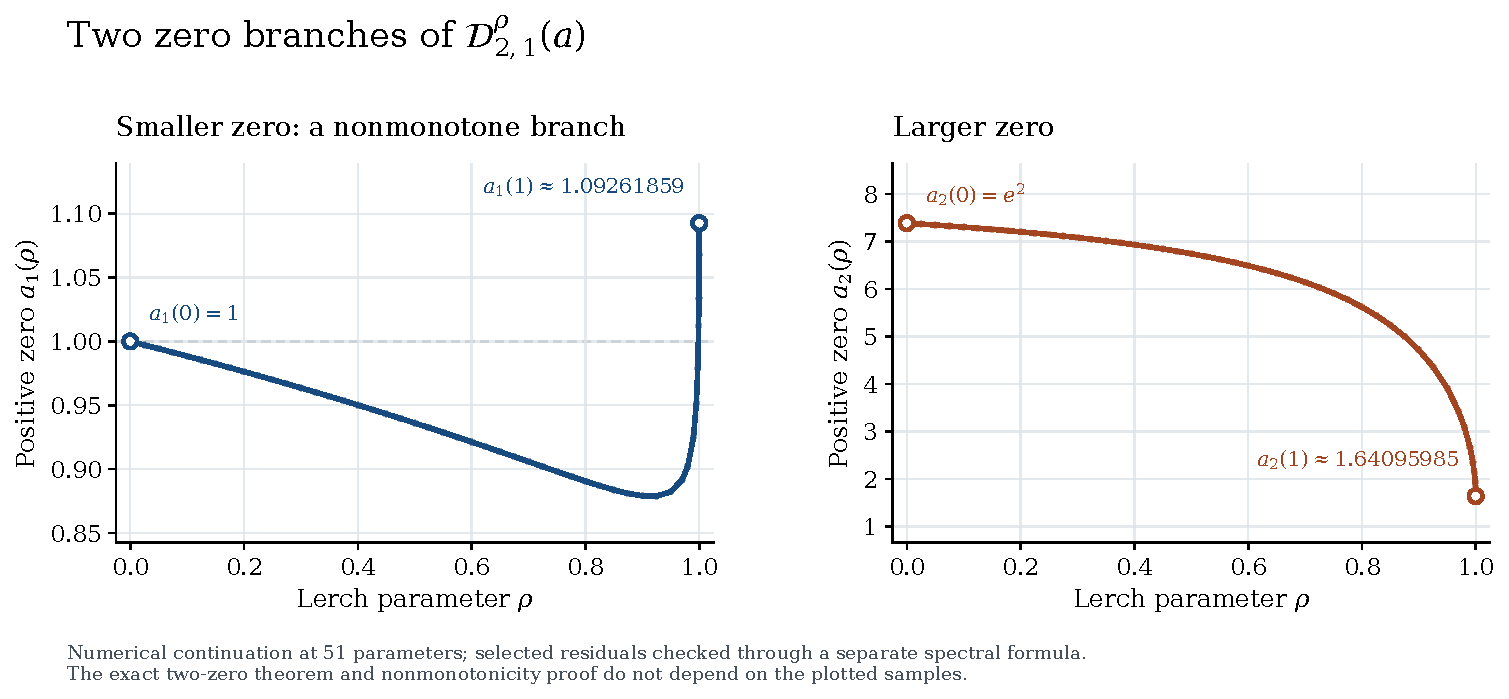
\includegraphics[width=\linewidth]{figures/lerch_n2_branches.pdf}
\caption{The two positive zeros of $\mathcal D_{2,1}^{\rho}(a)$,
computed at $51$ parameter values. The first branch is nonmonotone;
the second joins $e^2$ to approximately $1.6409598465$.
The curves and interior locations are numerical diagnostics. The
existence, simplicity, exact zero count, and nonmonotonicity of the
first branch follow independently from the proofs.}
\label{lerchboundary:fig:two-branches}
\end{figure}

The endpoint roots are numerically
$a_1(1)\approx1.0926185942922162563$ and
$a_2(1)\approx1.6409598465375973621$. Among the plotted samples, the
smallest first-branch value occurs at $\rho=0.925$, with
$a_1\approx0.878826386000143658$. This is a sampled minimum, not a
certified optimizer. The largest Laplace residual of the $102$ roots
is below $5.60\times10^{-30}$; $14$ independent Lerch/Hurwitz spectral
checks have residuals below $3.13\times10^{-30}$. Numerical rounding
is not interval-certified.

% END sections/lerch_zeros
% BEGIN sections/lerch_shape
% Add after the global n=2 two-zero theorem in lerch_boundary_notes.tex.
% No numerical input beyond the exact endpoint sign already certified there.

\subsection{Monotonicity of the larger branch and a unique level crossing}
\label{lerchshape:sec:n2}

The single change of coefficient sign also determines the shape of the
larger zero branch and the part of the smaller branch above $a=1$.
These conclusions leave a sharper question about the number of extrema
of the smaller branch below this level.

\begin{corollary}[Shape constraints for the two zero branches]
\label{lerchshape:cor:n2}
Let $a_1(\rho)<a_2(\rho)$ be the two simple positive zeros in
Theorem~\ref{lerchboundary:thm:n2global}. Then $a_2$ is strictly
decreasing on $[0,1]$, with
\[
 \frac{13}{10}<a_2(\rho)<e^2\qquad(0<\rho\leq1),
 \qquad a_2(0)=e^2.
\]
There is a unique $\rho_c\in(0,1)$ such that $a_1(\rho_c)=1$.
Moreover,
\[
 a_1(\rho)<1\quad(0<\rho<\rho_c),\qquad
 a_1(\rho)>1\quad(\rho_c<\rho\leq1),
\]
and
\[
 a_1'(\rho)>0\quad(\rho_c\leq\rho<1),\qquad
 a_2'(\rho)<0\quad(0<\rho<1).
\]
In particular, the level crossing is transverse, and every interior
critical point of $a_1$ lies in $(0,\rho_c)$.
\end{corollary}

\begin{proof}
Write $G=G_{2,1}$ and
\[
 f(u)=\frac{\log u(\log u-2)}{u^2},\qquad
 G(a,\rho)=\sum_{m=0}^{\infty}\rho^m f(a+m).
\]
For a fixed $a\in[1,e^2)$ set $c=e^2-a>0$ and $b_m=f(a+m)$.
The coefficient $b_m$ is nonpositive for $m<c$ and nonnegative
for $m>c$, and it vanishes if $m=c$. Thus
\[
 (m-c)b_m\geq0\qquad(m\geq0).
\]
There are strictly positive terms, for example every integer $m>c$.
Termwise differentiation is valid for $0<\rho<1$, and gives the
strict differential inequality
\begin{equation}\label{lerchshape:eq:weighted}
 \rho G_\rho(a,\rho)-cG(a,\rho)
   =\sum_{m=0}^{\infty}(m-c)b_m\rho^m>0.
\end{equation}
The use of a real cutoff $c$ includes without exception the possibility
that one coefficient vanishes at $a+m=e^2$.

For $\rho>0$, the $m=0$ term at $a=e^2$ vanishes and all terms with
$m\geq1$ are positive. Therefore $G(e^2,\rho)>0$. Together with
$G(13/10,\rho)<0$ and the two-zero theorem, this places the larger
zero in $(13/10,e^2)$, including at $\rho=1$. The signs at the
simple zeros are
\[
 G_a(a_1(\rho),\rho)<0,
 \qquad G_a(a_2(\rho),\rho)>0,
\]
since $G$ is positive before the smaller zero, negative between
the two zeros, and positive after the larger zero. At any zero
in $[1,e^2)$, \eqref{lerchshape:eq:weighted} gives $G_\rho>0$.
Implicit differentiation consequently gives $a_2'=-G_\rho/G_a<0$
for $0<\rho<1$. Continuity at both endpoints proves strict decrease
on the whole closed interval.

Now fix $a=1$ and put $c_0=e^2-1$. The same inequality shows that
\[
 \frac{d}{d\rho}\bigl(\rho^{-c_0}G(1,\rho)\bigr)
 =\rho^{-c_0-1}\bigl(\rho G_\rho(1,\rho)-c_0G(1,\rho)\bigr)>0
 \qquad(0<\rho<1).
\]
The expression is continuous up to $\rho=1$. Since $f(1)=0$ and
$f(2)<0$, one has $G(1,\rho)=\rho f(2)+O(\rho^2)<0$ for small
positive $\rho$. The exact certificate
\eqref{lerchboundary:eq:n2cert-one} gives $G(1,1)>0$.
Strict increase of the weighted expression therefore gives precisely
one zero $\rho_c\in(0,1)$, with negative sign before and positive
sign after it.

Because $1<13/10<a_2(\rho)$, the sign of $G(1,\rho)$ is negative
exactly when $a_1(\rho)<1$, and positive exactly when $a_1(\rho)>1$.
This proves the asserted unique crossing and the inequalities on
each side. When $\rho_c\leq\rho<1$, the smaller root lies in
$[1,13/10)$, so \eqref{lerchshape:eq:weighted} applies there as well.
Its negative $a$ derivative now gives $a_1'=-G_\rho/G_a>0$,
including at the crossing itself.
\end{proof}

The remaining shape question is whether $a_1$ has exactly one minimum
in $(0,\rho_c)$; a sharper version asks whether its derivative has
exactly one zero there. Neither uniqueness assertion is required for
the corollary.
% END sections/lerch_shape
% BEGIN sections/lerch_abel
% Optional additional section. Uses G_{n,k} from lerch_boundary_notes.tex.

\section{The logarithmic singularity at the Stieltjes endpoint}
\label{lerchboundary:sec:abel}

The opposite endpoint $\rho=1$ is continuous for the differentiated
Lerch family, but it is not infinitely differentiable in its deformation
parameter.  The following elementary Abel estimate identifies the first
singular term and transfers it to every simple endpoint zero.  Its
logarithmic structure is the classical one for power-logarithm
Dirichlet coefficients; the point here is its precise normalization
and its consequence for zero branches.

Put $\tau=-\log\rho$ and $L=\log(1/\tau)$, so that
$\rho\uparrow1$ corresponds to $\tau\downarrow0$.  For
$0\leq j\leq k-1$ define the absolutely convergent moments
\begin{equation}\label{lerchboundary:eq:moments}
 \mu_j(a)=\sum_{m=0}^{\infty}m^j f_{n,k}(a+m),
 \qquad
 H(a,\tau)=\sum_{j=0}^{k-1}\frac{(-\tau)^j}{j!}\mu_j(a).
\end{equation}
For $j=0$ use $m^0=1$, including at $m=0$.

\begin{theorem}[The first singular Abel coefficient]
\label{lerchboundary:thm:abel}
Fix $n\geq1$, $k\geq1$, and a compact interval $I\subset(0,\infty)$.
Uniformly for $a\in I$, as $\tau\downarrow0$,
\begin{equation}\label{lerchboundary:eq:abel}
 G_{n,k}(a,e^{-\tau})=H(a,\tau)
 +\frac{(-1)^{n+k}}{k!(n+1)}\tau^k L^{n+1}
 +O_{n,k,I}(\tau^k L^n).
\end{equation}
The family has continuous one-sided derivatives in $\tau$ through
order $k-1$ at zero. Its next derivative satisfies
\begin{equation}\label{lerchboundary:eq:abel-derivative}
 \partial_\tau^kG_{n,k}(a,e^{-\tau})
 =\frac{(-1)^{n+k}}{n+1}L^{n+1}+O_{n,k,I}(L^n).
\end{equation}
In particular it has no finite continuous $k$th derivative there.
The leading singular coefficient is independent of $a$.
\end{theorem}

\begin{proof}
Monicity of $P_{n,k}$ and a uniform expansion at large $m$ give
\begin{equation}\label{lerchboundary:eq:tail-coefficient}
 f_{n,k}(a+m)
 =\frac{(-1)^n(\log m)^n}{m^{k+1}}
 +O_{n,k,I}\left(\frac{(1+\log m)^{n-1}}{m^{k+1}}\right),
 \qquad m\geq1.
\end{equation}
Each $a$-derivative adds a factor $O(m^{-1})$, apart from bounded-degree
logarithmic factors.  All moments in \eqref{lerchboundary:eq:moments}
therefore converge normally on positive compact $a$-sets, including
any fixed number of $a$-derivatives. Differentiation in $\tau$ up to
order $k-1$ is justified by dominated convergence.

Write
$R_{k-1}(x)=e^{-x}-\sum_{j=0}^{k-1}(-x)^j/j!$. For $0\leq x\leq1$,
\[
 R_{k-1}(x)=\frac{(-1)^k x^k}{k!}+O_k(x^{k+1}),
\]
and for $x\geq1$, $|R_{k-1}(x)|\leq C_k x^{k-1}$.
Subtract $H$ from the defining series for $G$ and split the sum at
$m=1/\tau$. The leading part of the lower range is
\[
 \frac{(-1)^{n+k}\tau^k}{k!}
 \sum_{1\leq m\leq1/\tau}\frac{(\log m)^n}{m}
 =\frac{(-1)^{n+k}\tau^k}{k!(n+1)}L^{n+1}+O_{n,k}(\tau^k).
\]
The Taylor remainder in that range is
$O(\tau^{k+1}\sum_{m\leq1/\tau}(1+\log m)^n)
=O(\tau^k L^n)$.  The lower-order coefficient term in
\eqref{lerchboundary:eq:tail-coefficient} contributes
$O(\tau^k\sum_{m\leq1/\tau}(1+\log m)^{n-1}/m)
=O(\tau^kL^n)$. Finally the upper range is bounded by
\[
 C\tau^{k-1}\sum_{m>1/\tau}\frac{(1+\log m)^n}{m^2}
 =O(\tau^kL^n).
\]
These bounds prove \eqref{lerchboundary:eq:abel}, uniformly in $a$.

To avoid differentiating a remainder, compute the next derivative
directly for $\tau>0$:
\[
 \partial_\tau^kG_{n,k}(a,e^{-\tau})
 =(-1)^k\sum_{m\geq1}m^k e^{-m\tau}f_{n,k}(a+m).
\]
Equation~\eqref{lerchboundary:eq:tail-coefficient}, the same cutoff,
and $|e^{-x}-1|\leq x$ for $0\leq x\leq1$ give
\[
 \sum_{m\geq1}\frac{e^{-m\tau}(\log m)^n}{m}
 =\frac{L^{n+1}}{n+1}+O_n(L^n).
\]
The lower logarithmic powers contribute $O(L^n)$.
This proves \eqref{lerchboundary:eq:abel-derivative} independently
of differentiation of \eqref{lerchboundary:eq:abel}.
\end{proof}

\begin{theorem}[Endpoint regularity and singular displacement of simple zeros]
\label{lerchboundary:thm:abel-root}
Let $r>0$ be a simple zero of $G_{n,k}(\cdot,1)$, and write
$q=\partial_aG_{n,k}(r,1)\neq0$.
There is a unique nearby real zero $a(\tau)$ of
$G_{n,k}(\cdot,e^{-\tau})$ for all sufficiently small $\tau\geq0$.
Let $\alpha(\tau)$ be the real analytic zero of $H(\cdot,\tau)$
through $\alpha(0)=r$. Then
\begin{equation}\label{lerchboundary:eq:abel-root}
 a(\tau)=\alpha(\tau)
 -\frac{(-1)^{n+k}}{k!(n+1)q}\tau^k L^{n+1}
 +O_{n,k,r}(\tau^kL^n).
\end{equation}
The branch is $C^{k-1}$, but not $C^k$, at the endpoint, in either
$\tau$ or $\rho$. Moreover
\begin{equation}\label{lerchboundary:eq:abel-root-derivative}
 \frac{d^k a}{d\tau^k}
 =-\frac{(-1)^{n+k}}{(n+1)q}L^{n+1}+O_{n,k,r}(L^n).
\end{equation}
\end{theorem}

\begin{proof}
Uniform convergence of $G$ and $G_a$, together with $q\neq0$, gives
one and only one zero near $r$, continuously in $\tau\geq0$.
The ordinary analytic implicit function theorem applies to the finite
polynomial $H$, since $H_a(r,0)=q$.
Evaluating \eqref{lerchboundary:eq:abel} at $\alpha(\tau)$ and using a
uniform lower bound for $|G_a|$ first gives
$a-\alpha=O(\tau^kL^{n+1})$.  Taylor expansion in $a$, followed by
$H_a(\alpha(\tau),\tau)=q+O(\tau)$, gives
\eqref{lerchboundary:eq:abel-root}; the quadratic error in the
displacement and the $O(\tau)$ change of the denominator are both
$O(\tau^kL^n)$.

The convergent differentiated series show that $G$ has all mixed
derivatives of total order at most $k-1$ continuously at the endpoint.
Implicit differentiation, or the one-sided implicit function theorem,
therefore gives $a\in C^{k-1}$. Differentiate the implicit identity
$k$ times for $\tau>0$.  Every mixed derivative involving at least
one $a$-derivative remains bounded, because that derivative improves
the spectral tail by one inverse power of $m$. All derivatives of
$a$ of order below $k$ have finite limits. Thus the only unbounded
term other than $G_a a^{(k)}$ is the pure $\tau$ derivative in
\eqref{lerchboundary:eq:abel-derivative}. Solving for $a^{(k)}$ proves
\eqref{lerchboundary:eq:abel-root-derivative}. In this step replacing
$G_a(a(\tau),e^{-\tau})$ by $q$ incurs only $O(L^n)$:
its difference is $O(\tau+|a(\tau)-r|)$, because $G_{a\tau}$ is
bounded at the endpoint, and
$|a(\tau)-r|=O(\tau+\tau^kL^{n+1})$.
The leading coefficient is nonzero, so the $k$th derivative has no
finite endpoint limit.  Finally $\tau=-\log\rho$ is a smooth local
change of variable with nonzero derivative at $\rho=1$.
\end{proof}

For the two branches of Theorem~\ref{lerchboundary:thm:n2global}, this
gives a particularly visible endpoint effect. If $r_i=a_i(1)$ and
$q_i=\partial_aG_{2,1}(r_i,1)$, then $q_1<0<q_2$ and
\[
 a_i(\rho)=r_i+\frac{\tau}{3q_i}L^3+O(\tau L^2),\qquad
 \frac{da_i}{d\rho}=-\frac{1}{3q_i}L^3+O(L^2).
\]
Thus $a_1'(\rho)\to+\infty$ and $a_2'(\rho)\to-\infty$ as
$\rho\uparrow1$.  The nonmonotonicity of $a_1$ already follows from
the elementary endpoint and the rational Stieltjes signs; this Abel
calculation supplies its quantitative endpoint behavior.
% END sections/lerch_abel
% BEGIN sections/angular_expansion
\section{A complete exponential expansion for the angular zero}
\label{angular:sec:main}

For integers $a\geq1$ and real $b>0$, write
\[
 H_j^{(b)}=\sum_{m=1}^j m^{-b},\qquad
 F_{a,b}(z)=\Li_{a,b}(z,1)
   =\sum_{n=2}^{\infty}\frac{H_{n-1}^{(b)}}{n^a}z^n.
\]
The signed-density theorem in the pinned manuscript
\cite[\texttt{signed:thm:unique-zero}]{ProveItSnapshot}
proves that $\Imag F_{a,b}(e^{i\theta})$ has exactly one zero
$\theta_{a,b}$ in the open upper semicircle, that it is simple, and
that $0<\theta_{a,b}<\pi/2$.  Its proof uses a zero-mass density
with one sign change and a strictly ordered Cauchy kernel.  The source
also proves a four-term expansion as $a\to\infty$, uniformly for
$b\geq1$, and explicitly leaves a systematic further expansion open.

We give every coefficient, with a remainder at any prescribed
exponential scale.  The result is uniform throughout $b>0$.  Only
the elementary bound
\begin{equation}\label{angular:eq:hbound}
 1\leq H_j^{(b)}\leq j\qquad(j\geq1,\ b>0)
\end{equation}
is needed for this stronger uniformity.  The expansion is complete in the asymptotic sense. Theorem
\ref{angular:thm:divergence} proves that its infinite untruncated sum
diverges at every fixed $a,b$, even after equal bases are combined.

\subsection{The locally finite scale and its coefficients}

Let $\mathscr M$ be the set of nonzero finitely supported sequences
$\mathbf m=(m_3,m_4,\ldots)$ of nonnegative integers. Put
\[
 |\mathbf m|=\sum_{n\geq3}m_n,
 \qquad q(\mathbf m)=\prod_{n\geq3}(2/n)^{m_n}.
\]
For every $0<\eta<1$, only finitely many $\mathbf m$ have
$q(\mathbf m)>\eta$. Indeed, each occupied index satisfies
$n<2/\eta$, and $(2/3)^{|\mathbf m|}\geq q(\mathbf m)>\eta$ bounds
the total multiplicity. Distinct multisets can give the same rational
base: those coefficients must be added, not interpreted as distinct
asymptotic scales.

Define the analytic germ
\begin{equation}\label{angular:eq:phi}
 \phi_n(u)=-\frac{u\sin(n\pi/2-nu)}{\sin(2u)}\qquad(n\geq3),
\end{equation}
with its removable value at $u=0$. Its Taylor coefficients are rational.
For $k=|\mathbf m|$ define
\begin{equation}\label{angular:eq:coefficient}
 C_{\mathbf m}(b)=
 \frac{(k-1)!}{\prod_{n\geq3}m_n!}
 [u^{k-1}]\prod_{n\geq3}\phi_n(u)^{m_n}
 \prod_{n\geq3}\bigl(H_{n-1}^{(b)}\bigr)^{m_n}.
\end{equation}
Thus $C_{\mathbf m}(b)$ is an explicitly given rational polynomial
in finitely many generalized harmonic numbers. In particular it is
rational when $b$ is a positive integer.

\begin{theorem}[All exponential orders, uniformly in the second index]
\label{angular:thm:allorders}
For every fixed $0<\eta<1$, as the integer $a\to\infty$,
\begin{equation}\label{angular:eq:allorders}
 \delta_{a,b}:=\frac\pi2-\theta_{a,b}
 =\sum_{\substack{\mathbf m\in\mathscr M\\q(\mathbf m)>\eta}}
 C_{\mathbf m}(b)q(\mathbf m)^a+O_\eta(\eta^a),
\end{equation}
uniformly for all real $b>0$. The constant and the threshold for $a$
depend on $\eta$, but not on $b$. The coefficient vanishes whenever
the total multiplicity $\sum_{n\text{ odd}}m_n$ is even.
\end{theorem}

\begin{proof}
For $a\geq4$, the Fourier series and its first angular derivative
converge absolutely, uniformly under \eqref{angular:eq:hbound}.
The equation for the zero, normalized by $2^a$, is
\begin{equation}\label{angular:eq:fourier}
 S_{a,b}(\delta)=\sin(2\delta)+
 \sum_{n\geq3}H_{n-1}^{(b)}(2/n)^a
      \sin(n\pi/2-n\delta)=0.
\end{equation}
The $n=3$ term at $\delta=0$ is
$-H_2^{(b)}(2/3)^a$; the remaining nonzero terms there have
size $O((2/5)^a)$ uniformly in $b>0$.  On
$0\leq\delta\leq2(2/3)^a$, differentiating the series gives
\[
 S_{a,b}'(\delta)=2+O((2/3)^a).
\]
For example, the differentiated tail is bounded by
\[
 \sum_{n\geq3}n(n-1)(2/n)^a
 \leq (2/3)^a\sum_{n\geq3}n^2(3/n)^4,
\]
whose last sum is finite. The same elementary estimate bounds the
undifferentiated tails. Since $1\leq H_2^{(b)}\leq2$,
$S_{a,b}(0)<0<S_{a,b}(2(2/3)^a)$ for all sufficiently large $a$.
Consequently the zero in this interval is unique and
\begin{equation}\label{angular:eq:smallroot}
 \delta_{a,b}=O((2/3)^a),\qquad
 S_{a,b}'(\delta)\geq1
\end{equation}
there, uniformly in $b$. The source's global uniqueness identifies
this local root with $\pi/2-\theta_{a,b}$.

If $\eta\geq2/3$, the sum in \eqref{angular:eq:allorders} is empty
and \eqref{angular:eq:smallroot} proves the assertion.  Otherwise
take $N=\lceil2/\eta\rceil-1\geq3$ and keep only the modes
$3\leq n\leq N$ in \eqref{angular:eq:fourier}. On the real root
interval the omitted tail is bounded by
\begin{align*}
 \sum_{n>N}(n-1)(2/n)^a
 &\leq (2/(N+1))^a
       \sum_{n>N}(n-1)((N+1)/n)^4\\
 &=O_\eta(\eta^a).
\end{align*}
The derivative bounds give a unique small root $\delta_N$ of this
finite equation and
\begin{equation}\label{angular:eq:finiteerror}
 \delta_{a,b}-\delta_N=O_\eta(\eta^a).
\end{equation}
One can apply the mean value theorem between the two roots; both
are in a common interval where the derivative of the finite
equation is bounded below by $1$.

Now regard $z_3,\ldots,z_N$ as independent complex variables. The
finite equation
\[
 \sin(2\delta)+\sum_{n=3}^Nz_n\sin(n\pi/2-n\delta)=0
\]
has a holomorphic solution $\delta=\Psi_N(\mathbf z)$ near
$\mathbf z=0$, by the implicit function theorem with derivative $2$.
Dividing by $\sin(2\delta)/\delta$ gives
\[
 \delta=\sum_{n=3}^Nz_n\phi_n(\delta).
\]
Apply the finite-variable Lagrange--B\"urmann formula, or insert an
auxiliary scalar multiplying all $z_n$ and use the ordinary formula.
The coefficient of $\prod z_n^{m_n}$ is precisely
\[
 \frac{(k-1)!}{\prod m_n!}
 [u^{k-1}]\prod\phi_n(u)^{m_n}.
\]
This is a finite-variable use of classical Lagrange inversion;
Dirichlet-series inversion has a wider literature, for example
Kuznetsov~\cite{Kuznetsov2019}, but no infinite-variable convergence
theorem is being assumed here.

Choose $K$ so that $(2/3)^{K+1}\leq\eta$. Truncate the convergent
Taylor expansion of $\Psi_N$ at total degree $K$, then substitute
$z_n=H_{n-1}^{(b)}(2/n)^a$. Its Taylor remainder is
$O_\eta((2/3)^{(K+1)a})=O_\eta(\eta^a)$, uniformly by the finite
bounds $H_{n-1}^{(b)}\leq N$. Every discarded monomial whose
base is at most $\eta$ also has size $O_\eta(\eta^a)$.
Every multiset with base greater than $\eta$ is supported on
$\{3,\ldots,N\}$ and has total degree at most $K$. Combining
this observation with \eqref{angular:eq:finiteerror} proves
\eqref{angular:eq:allorders}.

Finally, $\phi_n$ is even in $u$ for odd $n$ and odd in $u$ for
even $n$. Its product can have a coefficient at $u^{k-1}$ only if
$\sum_{n\text{ even}}m_n\equiv k-1\pmod2$, equivalently if
$\sum_{n\text{ odd}}m_n$ is odd. This proves the vanishing assertion.
\end{proof}

\begin{remark}[Why the proof truncates the Fourier modes first]
The original Fourier series does not converge absolutely in a complex
neighborhood of a real angular argument: high frequencies grow on
one side of that neighborhood. An unqualified infinite-dimensional
analytic implicit-function argument would therefore leave a real gap.
The finite cutoff followed by a real derivative estimate avoids that
gap and proves exactly the asymptotic assertion stated above. Theorem~\ref{angular:thm:divergence} proves that the formal sum over
all multisets, and even the sum grouped by equal bases, diverges.
\end{remark}

\subsection{Ten terms and the next signed remainder}

Write $h_j=H_j^{(b)}$. Let $T_{10}(a,b)$ be the sum of $c(q)q^a$
over the ten rows in Table~\ref{angular:tab:ten}. The first four rows
recover the source's theorem. The next six and the uniformity for
all $b>0$ are supplied here.

\begin{table}[ht]
\centering
\caption{The complete angular expansion above the scale $(2/13)^a$.
Equal rational bases have already been combined.}
\label{angular:tab:ten}
\begin{tabular}{@{}cl@{}}
\toprule
$q$& $c(q)$ in $T_{10}=\sum c(q)q^a$\\
\midrule
$2/3$ & $h_2/2$\\
$2/5$ & $-h_4/2$\\
$1/3$ & $h_2h_3$\\
$8/27$ & $-23h_2^3/48$\\
$2/7$ & $h_6/2$\\
$2/9$ & $-(3h_2h_5+h_8)/2$\\
$1/5$ & $-h_3h_4$\\
$2/11$ & $h_{10}/2$\\
$8/45$ & $39h_2^2h_4/16$\\
$1/6$ & $2h_2(h_3^2+h_7)$\\
\bottomrule
\end{tabular}
\end{table}

\begin{corollary}[A sharp signed remainder after ten terms]
\label{angular:cor:ten}
Uniformly for $b>0$,
\begin{equation}\label{angular:eq:eleven}
 \delta_{a,b}=T_{10}(a,b)-\frac{h_{12}}2(2/13)^a
       +O((4/27)^a).
\end{equation}
In particular,
\[
 \frac{\delta_{a,b}-T_{10}(a,b)}{(2/13)^a}
   =-\frac{h_{12}}2+O((26/27)^a).
\]
For all sufficiently large integer $a$, with a threshold independent
of $b>0$, the ten-term approximation strictly overestimates
$\delta_{a,b}$ and therefore gives a strict lower approximation to
$\theta_{a,b}$.
\end{corollary}

\begin{proof}
Apply Theorem~\ref{angular:thm:allorders} at the cutoff $4/27$.
The only additional nonzero base strictly between $4/27$ and
$2/13$, including $2/13$ itself, is $2/13$ with coefficient
$-h_{12}/2$.  This finite assertion can be checked by the multiset
bounds in the proof, or by the exact generator supplied with the
article.  The source four-term coefficient and all six new displayed
coefficients are also verified by substitution into the original
Fourier equation, independently of the Lagrange coefficient formula.
Finally $h_{12}\geq1$, so the uniform remainder gives the eventual
strict sign.
\end{proof}

For illustration, at $a=256$, $b=4$, direct Fourier root evaluation
gives
\[
 \delta_{256,4}\approx4.42523791578002118187450681399\times10^{-46}.
\]
The ten-term absolute error is approximately $4.24289006845\times10^{-209}$.
Its normalized error is $-0.541353663458730256$, approaching the
predicted limit
\[
 -H_{12}^{(4)}/2=-0.541076555073967515\ldots.
\]
The convergence of this last ratio is deliberately slow: its proved
next scale is $(26/27)^a$.  These decimal values are independent
high-precision diagnostics, not interval certificates or inputs to
the proof.  The supplied script bounds the omitted Fourier tail and
labels its floating-point status explicitly.

The next coefficient can also be made explicit. Extraction through the
cutoff $1/7$ gives
\begin{align*}
 \delta_{a,b}={}&T_{10}(a,b)-\frac{h_{12}}2(2/13)^a
 -\frac{27}{8}h_2^3h_3(4/27)^a+O((1/7)^a),
\end{align*}
uniformly for $b>0$. The nonzero contribution at base $4/27$ comes
from the multiset $(3,3,3,4)$; the other representations vanish by
parity. The accompanying audit extraction substitutes all twelve
terms back into the Fourier equation with exactly zero surviving
residual above the cutoff. This extra negative term explains the
direction of approach of the normalized numerical error.

\subsection{An exact and finite coefficient algorithm}

To compute the expansion above a prescribed rational cutoff $\eta$,
enumerate nondecreasing multisets of integers $n\geq3$ while
$\prod(2/n)>\eta$.  The total multiplicity and the possible indices
are bounded as in the theorem. Remove multisets containing an even
number of odd indices. Compute the coefficient in
\eqref{angular:eq:coefficient} with exact polynomial arithmetic and
combine equal rational bases. This algorithm terminates for every
cutoff, uses no integer-relation search, and returns the complete
coefficient set at that scale.

For the cutoff $2/13$, it examines 25 multisets and produces the ten
nonzero combined bases in Table~\ref{angular:tab:ten}. The verification
routine then substitutes the answer into \eqref{angular:eq:fourier}
in a separately implemented finite algebra of rational exponential
bases. Every surviving coefficient cancels exactly. Thus the artifact
checks the coefficient identities, while the theorem proves the
uniform analytic remainder and the applicability of those identities
to the actual zero.
% END sections/angular_expansion
% BEGIN sections/angular_divergence
% Insert after the all-exponential-orders theorem and its proof.
% Uses the notation and coefficient formula of angular_transseries.tex.
\subsection{The complete exponential series diverges at every fixed index}
\label{angular:sec:divergence}

The finite-cutoff theorem cannot be strengthened to ordinary convergence
of the complete coefficient series. This obstruction persists after
all equal rational exponential bases have been combined.
For a base $q$, put
\[
 \widehat C(q;b)=\sum_{\mathbf m:\,q(\mathbf m)=q}C_{\mathbf m}(b).
\]
Each such sum is finite by local finiteness of the scale.

\begin{theorem}[Divergence after grouping equal bases]
\label{angular:thm:divergence}
For every fixed integer $a\ge1$ and real $b>0$, the ordinary series
\[
 \sum_q\widehat C(q;b)q^a
\]
does not converge. In fact its individual terms are unbounded along
an infinite sequence of distinct rational bases tending to zero.
The ungrouped multiset series also diverges. Thus the complete
expansion in Theorem~\ref{angular:thm:allorders} is asymptotic and
necessarily divergent at every fixed $a,b$.
\end{theorem}
\begin{proof}
Choose an integer $s\ge1$ with $2s>a$, and put $K=2s+1$.
For an odd prime $P\ne3$, consider the multiset with $2s$ copies
of $3$ and one copy of $P$. Its base is
\begin{equation}\label{angular:eq:prime-base}
 q_P=\frac{2^K}{3^{2s}P}.
\end{equation}
We first prove that this base has no other multiset representation.
If $k$ integers $n_1,\ldots,n_k\ge3$ give the same base, then
\[
 \prod_{j=1}^k n_j=2^{k-K}3^{2s}P.
\]
Since the left side is an integer and $3^{2s}P$ is odd, $k\ge K$.
Let $\Omega(n)$ denote the number of prime factors of $n$, with
multiplicity. Additivity gives
\[
 \sum_{j=1}^k\Omega(n_j)=(k-K)+2s+1=k.
\]
Each summand is at least one, so every $n_j$ is prime. The lower
bound $n_j\ge3$ excludes the prime two; hence $k=K$, and unique
factorization leaves precisely $2s$ copies of $3$ and one copy
of $P$. Therefore $\widehat C(q_P;b)$ is exactly the coefficient
of this one multiset, with no possible cancellation from other
representations.

Write $h_j=H_j^{(b)}$, let $\sigma_P=\sin(P\pi/2)\in\{-1,1\}$,
and introduce the even analytic germ
\[
 B(u)=\frac{u}{\sin(2u)},\qquad B(0)=\frac12.
\]
For odd $P$, the coefficient germs in
\eqref{angular:eq:phi} satisfy
\[
 \phi_3(u)=B(u)\cos(3u),\qquad
 \phi_P(u)=-\sigma_P B(u)\cos(Pu).
\]
The multinomial prefactor in \eqref{angular:eq:coefficient} is
$(K-1)!/((2s)!1!)=1$. Consequently
\begin{align}
 \widehat C(q_P;b)
 &=-\sigma_Ph_2^{2s}h_{P-1}\,\mathcal P_s(P),
 \label{angular:eq:prime-coefficient}\\
 \mathcal P_s(P)
 &:=[u^{2s}]B(u)^{2s+1}\cos^{2s}(3u)\cos(Pu)
 \notag\\
 &=\frac{(-1)^s}{2^{2s+1}(2s)!}P^{2s}
     +O_s(P^{2s-2}).
 \label{angular:eq:prime-polynomial}
\end{align}
The last equality is a polynomial identity in $P$ followed by its
leading-term estimate. Its highest power comes only from the
$u^{2s}$ coefficient of $\cos(Pu)$ and the constant coefficient
$2^{-2s-1}$ of the remaining factor. All other powers are even
and at most $2s-2$.

Combining \eqref{angular:eq:prime-base} and
\eqref{angular:eq:prime-polynomial} gives, along odd primes,
\[
 \bigl|\widehat C(q_P;b)q_P^a\bigr|
 =\frac{2^{K(a-1)}h_2^{2s}}{3^{2sa}(2s)!}
   h_{P-1}P^{2s-a}\bigl(1+O_s(P^{-2})\bigr).
\]
Here $h_{P-1}\ge1$. Since $2s-a>0$, these terms tend to infinity
as $P\to\infty$ through odd primes different from three. Such
primes are infinite; no estimate for their distribution is needed.
The bases $q_P$ are distinct and tend to zero. The necessary
condition that individual summands tend to zero therefore fails,
both for the grouped series and for the ungrouped series, and
indeed for every ordering of these ordinary series.
\end{proof}

For example, the first two polynomials in
\eqref{angular:eq:prime-polynomial} are
\[
 \mathcal P_1(P)=-\frac{P^2+14}{16},\qquad
 \mathcal P_2(P)=\frac{P^4}{768}+\frac{11P^2}{48}
                   +\frac{81}{32}.
\]
The supplied script \texttt{check\_angular\_divergence.py} computes
these coefficient polynomials exactly through $s=6$, checks their
leading coefficients, and compares six small cases with direct
symbolic trigonometric expansion. The general proof above, not
these finite checks, establishes divergence.

There is no conflict with the complete asymptotic theorem. Its
cutoff is fixed first and then $a$ tends to infinity. The divergent
subsequence above fixes $a$ first and lets the retained frequency
grow without bound. Summation procedures beyond ordinary series
convergence are a separate question.
% END sections/angular_divergence
% BEGIN sections/audit
\section{Audit findings and proposed manuscript corrections}
\label{audit:sec:corrections}

The research does not require withdrawing the source's global zero
bound, its eventual uniform saturation theorem, its $n=1$ monotonicity
theorem, or its all-conductor symbol kernel theorem. Those results
survive the present analysis. The following corrections and status
updates are narrower and should be integrated with their supporting
proofs.

\subsection{A logical wording correction in the rank conjecture}

In \path{chapters/05-signed-kernels.tex}, Conjecture
\texttt{signed:conj:rank} states two absolute ranks and then describes
their difference as an equivalent statement. The difference follows
from the two absolute formulas, but it does not recover them without
another premise. Replace ``Equivalently'' by ``Consequently'' and
``The equivalence'' by ``This implication.'' This is a logical wording
correction, independent of whether the conjecture is true. Theorem
\ref{fg:thm:rank} now proves both absolute ranks, so after its proof
has been integrated the conjecture can be promoted to a theorem.

The attached patch makes only those wording changes and the duplicated
phrase correction below. It deliberately leaves the conjecture
environment intact: installing a new theorem label without its proof
and dependencies would be a poor intermediate repository state.

\subsection{Boundary regularization must remain explicit}

The removed coordinate $X_1^{0,1}$ and the retained difference row are
essential parts of the matrix definition. A computation that discards
both boundary rows, or retains them separately as homogeneous rows,
solves a different problem. The canonical defect $cY^n$ in Lemma
\ref{fg:lem:boundary} identifies exactly what the valid regularization
preserves. The matrix generator includes column order, row labels, and
the weight-five matrix itself so future implementations can compare
the actual presentation, not merely a rank value.

Similarly, the new universal splitting concerns only the specified
single-product coefficient system. Adding distribution or higher-depth
relations can change the residual kernel. The theorem should not be
paraphrased as a numerical dimension conjecture for all cyclotomic
multiple polylogarithms.

\subsection{The angular expansion is no longer an open construction}

The paragraph following the source's angular numerical table describes
a systematic expansion beyond four terms as a separate research
problem. Theorem~\ref{angular:thm:allorders} resolves that problem at
every fixed exponential accuracy, and extends the uniformity from
$b\geq1$ to $b>0$. The correct replacement should also mention
Theorem~\ref{angular:thm:divergence}: the infinite grouped series has
unbounded terms at fixed $a,b$. Ordinary convergence is therefore
ruled out, not merely unproved.

An analytic implicit-function argument on the entire complex Fourier
series would be invalid without additional work: its frequencies grow
exponentially off the real axis. The finite-mode argument in this
article is part of the proof, not an implementation detail that may
be dropped from an abbreviated presentation.

\subsection{Higher-index monotonicity needs counterexamples, not extrapolation}

The source proves a decreasing branch at $n=1$. It does not thereby
prove decreasing branches at larger indices. Theorem
\ref{lerchboundary:thm:counterexample} gives a strictly positive initial
velocity for the smallest $n=4,k=3$ branch. Theorem
\ref{lerchboundary:thm:n2global} gives an entire $n=2,k=1$ branch that
is nonmonotone on $[0,1]$. These are useful additions to the discussion
of higher-index motion; they do not contradict the correctly restricted
$n=1$ theorem.

The regularity statement must distinguish the two endpoints. At a
simple elementary zero, analytic dependence on $\rho$ extends through
$0$. At a simple Stieltjes endpoint zero, Theorem
\ref{lerchboundary:thm:abel-root} gives exactly $C^{k-1}$ regularity,
with a divergent $k$th derivative. An unqualified claim of analyticity
on a neighborhood of the closed parameter interval would be false.

In the proof of the source result \texttt{half:zero:first}, replace
``The endpoint signs in the endpoint signs and the Laplace representation
above'' by ``The endpoint signs and the Laplace representation above.''
This is an editorial duplication only.

\subsection{Formal Herglotz obstructions and analytic evaluations}

The general companion classification must retain the condition modulo
$2e$. For example, the pair $e=8,o=3$ passes the corresponding tests
modulo $o$ and $e$, but fails $o^2\equiv1\pmod{2e}$. A criterion that
simply reuses the two moduli from the source's $F$-classification would
give an incorrect answer for $J(3/8)$.

The term ``no reduction'' in this setting means no reduction of the
specified invariant pre-Bloch element. The boundary argument is not
a transcendence theorem for actual values of $J$. Conversely, the
positive cases of the formal theorem ensure existence in the stated
calculus; they need not provide a short explicit logarithmic formula
until a constructive five-term reduction is supplied. The consecutive
family and $3/5$ evaluation provide such explicit analytic formulas
in useful cases.

The adjacent-argument functional identity used for these evaluations
is an independently derived reformulation of the known Choie--Kumar
functional equation \cite[Theorem 3.2(1)]{ChoieKumar2023}. It should be
credited accordingly. We do not claim priority for a general functional
equation already present in that paper. The inspected follow-up work
on character-weighted Herglotz integrals supplies relevant future
directions \cite{DixitSathyanarayanaSharan2024}.

\subsection{Status synchronization across incoming reports}

The recent rigidity report already proves the $S_4$ identity by an
explicit combination of standard rows and a Möbius-duality row
\cite{PriorRigidity}. Older descriptions of $S_4$ as an unresolved
global identity should be updated when that report is integrated.
The earlier obstruction for a smaller relation space remains a valid
statement about that smaller space. It should be preserved with its
scope, not treated as a contradiction to the later proof.

Likewise, the residual level-three and level-four invariant spaces
were computed in the preceding report \cite{PriorResearch}. The
new contribution is the free same-point lift and the full ranks under
the manuscript's exact boundary convention. The supplied integration
guide records this dependency to avoid duplicate priority claims.
% END sections/audit
% BEGIN sections/research
\section{A proposed research program}
\label{research:sec:program}

The results suggest concrete next problems. They are ordered by their
direct dependence on the new structure, rather than by a claim that
every direction has equal difficulty. Statements phrased as questions
below are not theorems of this article.

\subsection{Cyclotomic coefficient systems}

\paragraph{1. Determine the residual kernel at general level.}
Theorem~\ref{fg:thm:universal} removes every same-point sector
canonically. What is the remaining Hilbert series of
$\ker A_{N,w}^{\neg g}$ for fixed $N$? At levels three and four,
linear substitutions reduce the problem to small reflection groups.
At levels five, six, and eight, the next step is to write the remaining
color-polynomial equations, decompose them under color automorphisms,
and look for a finite invariant-theoretic presentation. Exact matrices
are valuable for selecting a candidate Hilbert series, but a proof
must identify generators, relations, and all boundary defects.

\paragraph{2. Add distribution without losing the canonical boundary data.}
Which of the free sectors survive when distribution rows are added?
The universal lift is supported on three colors per root pair, which
makes the image of each distribution row explicitly computable.
A useful first result would be a closed formula for the rank increment
at prime-power levels. This would also clarify the relation between
the coefficient systems here and the broader standard-relation spaces
of \cite{Zhao2010}.

\paragraph{3. Construct short relation certificates from the explicit dual basis.}
The nullspace test decides whether a proposed row is derivable, but
does not by itself minimize the number or coefficient height of the
rows used in a proof. Can the polynomial normal form be upgraded to
a constructive reduction algorithm whose certificate length is
polynomial in the weight? The existing $S_4$ certificate shows why
the choice of extra argument transformations matters. A principled
comparison between short certificates and large eliminated systems
would be useful for future repository formalization.

\subsection{Formal and analytic Herglotz arithmetic}

\paragraph{4. Make every positive classification case constructive.}
The congruence test answers whether the invariant companion symbol
vanishes, but a Bloch-group descent argument does not necessarily
produce a compact five-term derivation. Find an explicit logarithmic
formula, with a controllable number of terms, for all even--odd pairs
obeying the two congruences. The families
$J(e/(e^2-1))$ and $J(e/(e^2+1))$ are natural first targets beyond
consecutive arguments. Their formal reductions are proved here;
their simplest analytic evaluations remain to be found.

\paragraph{5. Classify subfield descent for combinations of symbols.}
An individual nonzero $\beta_M(a)$ cannot descend to a proper real
subfield, but combinations can. Character decomposition of the Gram
image should classify which coefficient vectors yield an element of
$\Lambda^2A(E)$ for a prescribed real subfield $E$. A complete answer
would generalize the denominator-rank formula and could distinguish
the smallest field needed by an explicit reduction from the ambient
cyclotomic field.

\paragraph{6. Complete the rank problem for companion values at fixed denominator.}
Theorem~\ref{jnew:thm:denominator-rank} gives an exact denominator
obstruction rank and a corresponding lower bound for formal companion
values modulo rational dilogarithms. What additional rank is supplied
by the numerator-conductor blocks? A useful formulation should fix a
finite numerator set and a common cyclotomic field, then compute the
intersection of the norm kernels. It should not confuse independence
in a symbol space with numerical independence of the evaluated periods.

\paragraph{7. Replace the dyadic difference by other Hecke combinations.}
The proof uses a cyclic Laplacian for multiplication by $2$ and a
quadratic field norm between adjacent dyadic conductors. Analogous
operators for an odd prime should interact with the Hecke functional
equations of \cite{RadchenkoZagier} and the character-weighted integrals
of \cite{DixitSathyanarayanaSharan2024}. Identify a natural companion
whose formal reduction is governed by a similarly explicit group
operator, and determine its exact kernel. The first challenge is to
keep rational wedge terms and conductor cancellation visible.

\subsection{Lerch bifurcations and uniform zero counts}

\paragraph{8. Prove or disprove uniqueness of the two-zero branch minimum.}
The smaller $n=2,k=1$ branch has at least one interior minimum and
an endpoint slope tending to $+\infty$. Does it have exactly one
critical point? Corollary~\ref{lerchshape:cor:n2} proves that the
larger branch is strictly decreasing, and that the smaller branch
increases after its unique crossing of $a=1$. The remaining question
therefore concerns only its motion below $1$. Differentiating the implicit equation gives
$a'=-G_\rho/G_a$; hence the first question reduces to the number of
solutions of $G=G_\rho=0$ on the first branch. A proof would require
a new sign-variation statement for this pair of kernels. A visually
single turn in the diagnostic plot is not enough to settle it.

\begin{conjecture}[Unique stationary point of the smaller branch]
\label{research:conj:minimum}
For $n=2,k=1$, the derivative $a_1'(\rho)$ vanishes at exactly one
point of $(0,1)$.
\end{conjecture}
The proved endpoint signs and Corollary~\ref{lerchshape:cor:n2}
would then identify that point as the unique global minimum, below
$\rho_c$. The numerical curve motivates the conjecture; no global
exclusion of additional stationary points is asserted here.

\paragraph{9. Locate and classify the forced interior events at $n=3,4$.}
At $k=1$, the small-$\rho$ counts and the certified $\rho=1$ counts
differ by two. We prove that an interior multiple zero occurs.
Determine whether there is exactly one event, and whether it is a
nondegenerate saddle-node, by certifying
\[
G=G_a=0,\qquad G_{aa}\ne0,\qquad G_\rho\ne0.
\]
Interval Newton or a two-variable argument principle could locate a
candidate, but global exclusion of further events must be supplied
separately. The current theorem deliberately makes no unverified
nondegeneracy claim.

\paragraph{10. Determine the optimal uniform threshold $K_n$.}
The present result gives $K_2=1$. The elementary endpoint forces
$K_n\geq n-1$: when $k<n-1$, the zero at $a=1$ is multiple and
uniform saturation by $n$ simple zeros fails at $\rho=0$.
The natural sharp question is whether $K_n=n-1$ for every $n\geq2$.
This equality is a candidate to test, not a conclusion of the existing
large-$k$ theorem. Exact sign certificates at selected separating
points, extended uniformly in $\rho$ by coefficient-sign arguments,
could prove the first new cases. A counterexample would reveal where
an interior loss of simplicity first occurs after the elementary
endpoint has already split completely.

\paragraph{11. Make the small-parameter classification effective in both indices.}
The sign of $\Delta_{n,k}$ is decidable by exact rational intervals
for $\log2$, but the proof gives no uniform lower bound for its
magnitude and no numerical value of $\rho_{n,k}$. Can one estimate
the distances of the roots of $P_{n,k}$ from $-\log2$ when $n,k$
grow? Such an estimate, together with a quantitative Rouché argument,
would turn the local classification into an explicit parameter range.
The resulting sign diagram may have a useful asymptotic description
when $k/n$ tends to a fixed ratio.

\paragraph{12. Compute the full Abel expansion of the zero branches.}
The leading singular coefficient is independent of $a$, while later
coefficients involve the tail expansion of $f_{n,k}(a+m)$ and the
regular moments. Derive the complete expansion in powers of $\tau$
and $\log\tau$, including collision terms from implicit inversion.
A particularly useful outcome would be a renormalized branch whose
successive singular terms can be subtracted algorithmically, with an
explicit differentiable remainder. This would also improve numerical
continuation near $\rho=1$.

\subsection{Divergent angular expansions}

\paragraph{13. Determine optimal truncation and the smallest attainable error.}
Theorem~\ref{angular:thm:allorders} keeps the cutoff fixed as
$a\to\infty$, whereas Theorem~\ref{angular:thm:divergence} rules out
ordinary convergence at fixed $a$. The next problem is quantitative:
how should the cutoff depend on $a$ to minimize the remainder, and
what is the resulting error scale? The proof must control the growth
of the finite implicit-function constants as the number of retained
modes increases. The prime-frequency obstruction supplies explicit
large coefficients and should constrain any proposed optimal rule.

\paragraph{14. Find a justified summation procedure.}
Can one recover the actual angular zero from the divergent coefficient
family by a natural summation method? Possible approaches include
keeping a finite Fourier equation exact while expanding only its low
modes, or reorganizing terms by a parameter introduced before the
mode cutoff. Any summability theorem must specify the order of
summation and explain why the unbounded grouped terms do not invalidate
the proposed procedure. A formal appeal to analyticity of the complete
Fourier series is insufficient.

\paragraph{15. Extend the angular theorem to other colors and depths.}
The current local root is governed by a dominant Fourier mode and
a nonzero real derivative, while the source's signed density proves
global uniqueness. Which depth-three or non-Gaussian color families
have both properties? Separate these two tasks: a local expansion can
be constructed before global uniqueness is known, but identifying it
with the intended geometric zero requires an independent global
argument. Multi-sign-change densities may produce several roots and
coupled singular limits, which would connect this direction with the
Lerch bifurcation analysis above.

\paragraph{A practical order of attack.}
The most immediate projects are the first residual levels in item~1,
constructive logarithmic evaluations in item~4, certified interior
events in item~9, and the first optimal-truncation estimates in item~13.
Each has a precise finite or analytic starting point supplied by this
article. The broader period-independence questions remain important,
but should be pursued with the formal-versus-numerical distinction
preserved at every stage.
% END sections/research
% BEGIN sections/verification
\section{Verification, artifacts, and integration procedure}
\label{verify:sec:reproduction}

The verification has two roles. Exact finite calculations check the
implementation of the displayed coefficient formulas, relation systems,
and rational signs. Independent numerical calculations test the analytic
evaluations and illustrate the geometry. Neither kind of computation
replaces the proofs for arbitrary indices or conductors.

\subsection{Exact coefficient and sign checks}

\begin{description}[style=nextline,leftmargin=0pt,labelwidth=0pt,labelsep=0pt]
\item[Gaussian ranks.]
The program \path{code/full_gaussian_rank.py} constructs the raw
shuffle and stuffle rows directly, including the boundary difference.
It independently performs rational elimination in weights $2$ through
$11$, checks the explicit integer nullvectors in selected weights
through $63$, and reproduces the source's $92\times23$ matrix at
weight five. Its receipt contains column order, row labels, the entire
weight-five matrix, and its kernel basis.

\item[Universal lift.]
The program \path{code/universal_gaussian_lift.py} generates the
cyclotomic rows afresh and verifies that the proposed lift annihilates
every row at levels $3,4,5,6,8,10,12$ in selected weights. It also
checks the rank differences by independent rational elimination in
weights $2,3,4$ at levels $3$ through $6$.

\item[Herglotz symbol calculations.]
The program \path{code/verify_j.py} performs $32{,}764$ exact
first- and second-difference zero tests at odd conductors through $401$.
Independent rational elimination checks the two spans, their common
rank, and the rank formula through conductor $101$. The program also
recovers the source's complete $J(2/q)$ classification from the general
criterion, and checks the arithmetic of the displayed infinite families.
These are integer group-algebra calculations; the logarithmic Gram
nonvanishing is supplied by the analytic theorem, not by a floating-point
determinant.

\item[Lerch polynomial identities and endpoint certificates.]
The program \path{code/verify_lerch_boundary.py} compares two exact
constructions of $P_{n,k}$ in $152$ cases. It computes $120$ rational
sign intervals for $\Delta_{n,k}$ through $n=16$ and certifies the
positive $n=4,k=3$ initial velocity. Eleven endpoint signs are replayed
using the source's outward-integer Euler--Maclaurin routine. Two signs
prove the $n=2$ separator and endpoint displacement; nine provide the
source's $n=3,4$ endpoint counts used to force interior multiple zeros.
The upstream routine is included verbatim with its original repository
path and SHA-256 recorded in the provenance data.

\item[Angular coefficients.]
The program \path{code/derive_angular.py} enumerates all rational
exponential bases above a requested cutoff, computes their Lagrange
coefficients exactly, combines collisions, and substitutes the result
into an independently coded Fourier expansion. The supplied cutoffs
$2/13$, $4/27$, $1/7$, and $1/10$ give respectively $10$, $11$, $12$,
and $20$ nonzero combined bases. Every surviving symbolic residual
vanishes exactly. The ten-term extraction examines $25$ multisets.

\item[Divergence coefficients.]
The program \path{code/check_angular_divergence.py} computes the
prime-frequency coefficient polynomials through $s=6$, verifies their
leading coefficients, and checks six cases against direct trigonometric
series expansion. Unique factorization and the general leading-term
argument establish divergence; the finite checks corroborate the
normalization.
\end{description}

\subsection{Independent numerical diagnostics}

The Herglotz verification uses $20$ independent integrations at $100$
decimal digits. For a positive rational $p/q$ it substitutes $t=s^q$,
so the integrand is
\[
q s^{q-1}\frac{\log(1+s^p)}{1+s^q}.
\]
It is regular at the lower endpoint and does not reuse the formula
being tested. The absolute acceptance tolerance is $10^{-85}$; the
largest observed residual in the supplied run is below $7\times10^{-100}$.
This is high-precision corroboration, not an interval certificate.

The angular diagnostic evaluates the real Fourier root in $15$ cases,
with $a=16,32,64,128,256$ and $b=1,2,4$. It uses exact quadrant
identities rather than subtracting trigonometric arguments close to
integer multiples of $\pi/2$. An analytic bound controls the omitted
Fourier tail; numerical rounding is not interval-enclosed. The theorem's
uniformity over every real $b>0$ follows from its proof, not from this
finite sample.

The two-zero figure is also numerical. Its data and generating script
are included, with independent spectral residual checks. The complete
zero count, nonmonotonicity, and endpoint regularity follow from the
proved sign and variation arguments independently of the plotted points.

\subsection{Rebuilding the contribution}

The archive has a single root directory. Its main components are
\path{article/}, \path{code/}, \path{data/}, \path{integration/}, and
\path{provenance/}. The complete source is
\path{article/main.tex}; a flattened source is also supplied as
\path{article/standalone.tex}. Both use the figures in
\path{article/figures/}. From the archive root:
\begin{verbatim}
python code/run_checks.py
make pdf
\end{verbatim}
The runner records package versions, script hashes, return codes, and
output hashes in \path{data/validation_receipt.json}. The Python
requirements are listed separately. The PDF build requires a standard
LaTeX installation with the packages declared in the preamble and
\texttt{latexmk}; no shell escape or network access is needed.
The optional figure reconstruction is documented in the README.

The PDF was compiled to a stable set of references and its rendered
pages were visually inspected. Package-level checks cover archive
integrity, presence of the stated artifacts, and checksums. These
checks concern the delivered files; they do not turn the mathematical
arguments into machine-checked proofs.

\subsection{Recommended integration order}

First apply the small editorial patch, which is independent of the new
proofs. Next integrate the Gaussian rank section with the universal
extension and its exact matrix generator. Integrate the Herglotz
classification before its denominator-rank and analytic corollaries.
For zero geometry, retain the existing global bound and insert the
elementary-endpoint, two-zero, and Abel-endpoint results in that order.
Finally replace the angular expansion's open-status paragraph with
the complete expansion and divergence theorems together.

The bibliography additions and the incoming-report status updates
should accompany those insertions. All new labels use the prefixes
\texttt{fg:}, \texttt{jnew:}, \texttt{lerchboundary:}, \texttt{lerchshape:}, and
\texttt{angular:}. The repository was not modified by this contribution;
the patch and fragments are proposed integration artifacts against the
pinned commit.
% END sections/verification
% BEGIN references
\begin{thebibliography}{99}
\raggedright
\addcontentsline{toc}{section}{References}

\bibitem{ProveItSnapshot}
V.~Reshetnikov and contributors, \emph{ProveIt: Analysis / Polylogarithms},
manuscript and research reports, repository snapshot of 10 October 2026,
commit \texttt{a2a4cf58c49c745058c40e4a6748d472a3420f18}.
\href{https://github.com/VladimirReshetnikov/ProveIt/tree/a2a4cf58c49c745058c40e4a6748d472a3420f18/Analysis/Polylogarithms/docs/manuscript}{Pinned manuscript snapshot on GitHub}.
The accompanying source manifest records the inspected chapter blobs.

\bibitem{PriorResearch}
ProveIt incoming research report,
\path{polylogarithms_research_2026-10-10.zip}, at the snapshot above.
In particular, the Gaussian section proves the residual level-three
and level-four polynomial descriptions used here.
\href{https://github.com/VladimirReshetnikov/ProveIt/tree/a2a4cf58c49c745058c40e4a6748d472a3420f18/Analysis/Polylogarithms/docs/incoming}{Incoming reports at the pinned snapshot}.

\bibitem{PriorRigidity}
ProveIt incoming research report,
\path{polylogarithms_rigidity_20261010.zip}, at the snapshot above.
In particular, the Gaussian section gives the Möbius-duality certificate
for $S_4$. The archive's Git blob is recorded in the incoming manifest.

\bibitem{Zhao2010}
J.~Zhao, \emph{Standard relations of multiple polylogarithm values at
roots of unity}, Documenta Mathematica \textbf{15} (2010), 1--34.
\url{https://arxiv.org/abs/0707.1459}.

\bibitem{Panzer2017}
E.~Panzer, \emph{The parity theorem for multiple polylogarithms},
Journal of Number Theory \textbf{172} (2017), 93--113.
\url{https://arxiv.org/abs/1512.04482}.

\bibitem{Umezawa2025}
R.~Umezawa, \emph{An explicit parity theorem for multiple polylogarithms},
arXiv:2508.02040 (2025).
\url{https://arxiv.org/abs/2508.02040}.

\bibitem{RadchenkoZagier}
D.~Radchenko and D.~Zagier,
\emph{Arithmetic properties of the Herglotz function},
Journal für die reine und angewandte Mathematik \textbf{797} (2023),
229--253.
\url{https://doi.org/10.1515/crelle-2023-0009}.
\url{https://arxiv.org/abs/2012.15805}.
Author manuscript:
\url{https://people.mpim-bonn.mpg.de/zagier/files/preprints/HerglotzFunction.pdf}.

\bibitem{ChoieKumar2023}
Y.~Choie and R.~Kumar,
\emph{Arithmetic properties of the Herglotz--Zagier--Novikov function},
Advances in Mathematics \textbf{433} (2023), Article 109315.
\url{https://doi.org/10.1016/j.aim.2023.109315}.
\url{https://arxiv.org/abs/2309.10634}.

\bibitem{DixitSathyanarayanaSharan2024}
A.~Dixit, S.~Sathyanarayana, and N.~Guru Sharan,
\emph{Mordell--Tornheim zeta functions and functional equations for
Herglotz--Zagier type functions}, arXiv:2405.07934 (2024).
\url{https://arxiv.org/abs/2405.07934}.

\bibitem{DLMFGamma}
NIST Digital Library of Mathematical Functions, Section 5.8,
\emph{Infinite products}, reciprocal-gamma Weierstrass product.
\url{https://dlmf.nist.gov/5.8}. Accessed 10 October 2026.

\bibitem{Lindemann1882}
F.~Lindemann, \emph{Ueber die Zahl $\pi$},
Mathematische Annalen \textbf{20} (1882), 213--225.
\url{https://doi.org/10.1007/BF01446522}.

\bibitem{Kuznetsov2019}
A.~Kuznetsov, \emph{Lagrange inversion theorem for Dirichlet series},
arXiv:1911.11133 (2019).
\url{https://arxiv.org/abs/1911.11133}.

\end{thebibliography}
% END references
\end{document}
